\documentclass{article}

% todo
% forum analysis
  % zotero export quote and reference it in the text
  % make a csv to read the entire forum
  % check a way of analysing into multiple categories

% observable
  % quantify the forum posts by categories, do a sitemap

% Notes
% Citation commands \cite \parencite \textcite 

% Useful packages
\usepackage[a4paper,top=2cm,bottom=2cm,left=3cm,right=3cm,marginparwidth=1.75cm]{geometry}
\usepackage{amsmath}
\usepackage{graphicx}
\graphicspath{{images/}}
\usepackage{svg}
\svgsetup{inkscapelatex=false} % - does not use the latex fonts in imported svg

\usepackage{lmodern}
\usepackage{array}  % Allows for more flexible column formatting
\usepackage{booktabs}  % Improves table aesthetics
\usepackage[skip=0.5ex, justification=raggedright, singlelinecheck=false]{caption}
\usepackage{enumitem}
\usepackage{float} % Required for the H specifier
\usepackage{subcaption} % Required for sub-figures

% table
\usepackage{multirow}
\usepackage{tabularx}
\usepackage{booktabs}


\PassOptionsToPackage{colorlinks=true, allcolors=blue}{hyperref}
\usepackage[style=apa, backend=biber]{biblatex}

\addbibresource{main.bib}

\newcommand{\getyear}[1]{\citeyear{#1}}
\usepackage{hyperref}

\DeclareCiteCommand{\fullcitefigure}
  {\boolfalse{citetracker}%
   \boolfalse{pagetracker}%
   \usebibmacro{prenote}}
  {\printtext{Photo by \printnames{author}, published in \printlist{organization} in \cite*{guptaBenFryConference2018}}%
   \renewcommand{\mkbibparens}[1]{} % Remove parentheses around citation
   \unspace\parencite{\thefield{entrykey}}} 
  {\multicitedelim}
  {\usebibmacro{postnote}}


% \title{Building and Sustaining Open Source Art Communities: Lessons from the Processing Project}
\title{Code, Community, and Creativity: Navigating the Complexities of Collective Contribution and Sustainability in the Processing Project}
\author{Tibor Udvari}



\begin{document}
\maketitle

\begin{abstract}
What are the dynamics that lead to the creation of a community around a piece of software? How do these dynamics influence the development of the software itself? This thesis explores these questions through the lens of the Processing community, a community of artists and designers who use the Processing software to create interactive art. The paper traces the history of the Processing community from its beginnings in 2001 to the present day, using a combination of interviews, archival research, and analysis of the software development cycle itself. The paper finds that the Processing community was created through a combination of factors, including the software's design, the community's shared values, and the community's shared history. The paper also finds that the community's shared history has influenced the development of the software itself, with the community's values and history influencing the software's design. The paper concludes by discussing the implications of these findings for the development of collaborative open source art software.
\end{abstract}

\newpage
%\tableofcontents

\section{Introduction}
% \subsection{The Background and Importance of Open Source Projects}
% -- about open source communities in general
% -- importance of open source projects, maybe mention how flash died out, and the recent unity price change ?

% todo NN - il faudrait des éléments visuels qui illustre mais aussi donne à voir ce qu’est Processing, et éventuellement là “où est la communauté”: des screenshots de forums, etc.

\subsection{The Processing Project: A brief overview}
% todo - adapt to focus more on the research question

Processing was developed as a programming language and environment specifically tailored for the media arts communities. Its inception took place at the MIT Media Lab's Aesthetics and Computation Group (ACG) in 2001, led by Ben Fry and Casey Reas. Its foundational concepts build upon the earlier work from the Design By Numbers (DBN) programming platform, a project spearheaded by John Maeda \parencite{fryModernPrometheusHistory2018}.

Ben Fry shed light on the holistic nature of the Processing initiative, noting:
\begin{quote}
"The processing project is a community, a piece of software that you run, and a language. And that order is important." – Ben Fry \parencite[19:22]{artsatmit2017CASTSymposium2017}
\end{quote}

In its design philosophy, Processing introduced the concept of "software sketches". It was designed with an accessible entry point for beginners, while also providing advanced capabilities for experienced users \parencite{reasProcessingProgrammingMedia2006}.

Over the years, Processing has been adopted across various disciplines, showcasing its versatility. To further its impact and development, the Processing Foundation was established, with notable contributors like Daniel Shiffman. The foundation aims to support and expand the reach of the Processing software and its associated projects.

% todo add
%\subsection{Objective and Scope of the Research}

% Choice of processing, because the community has been around for a while and the project is still alive and taught in schools, also at a high school level

% modular toolkit, not a monolith
% community, application, syntax
% commercial software


\begin{figure}
  \centering
  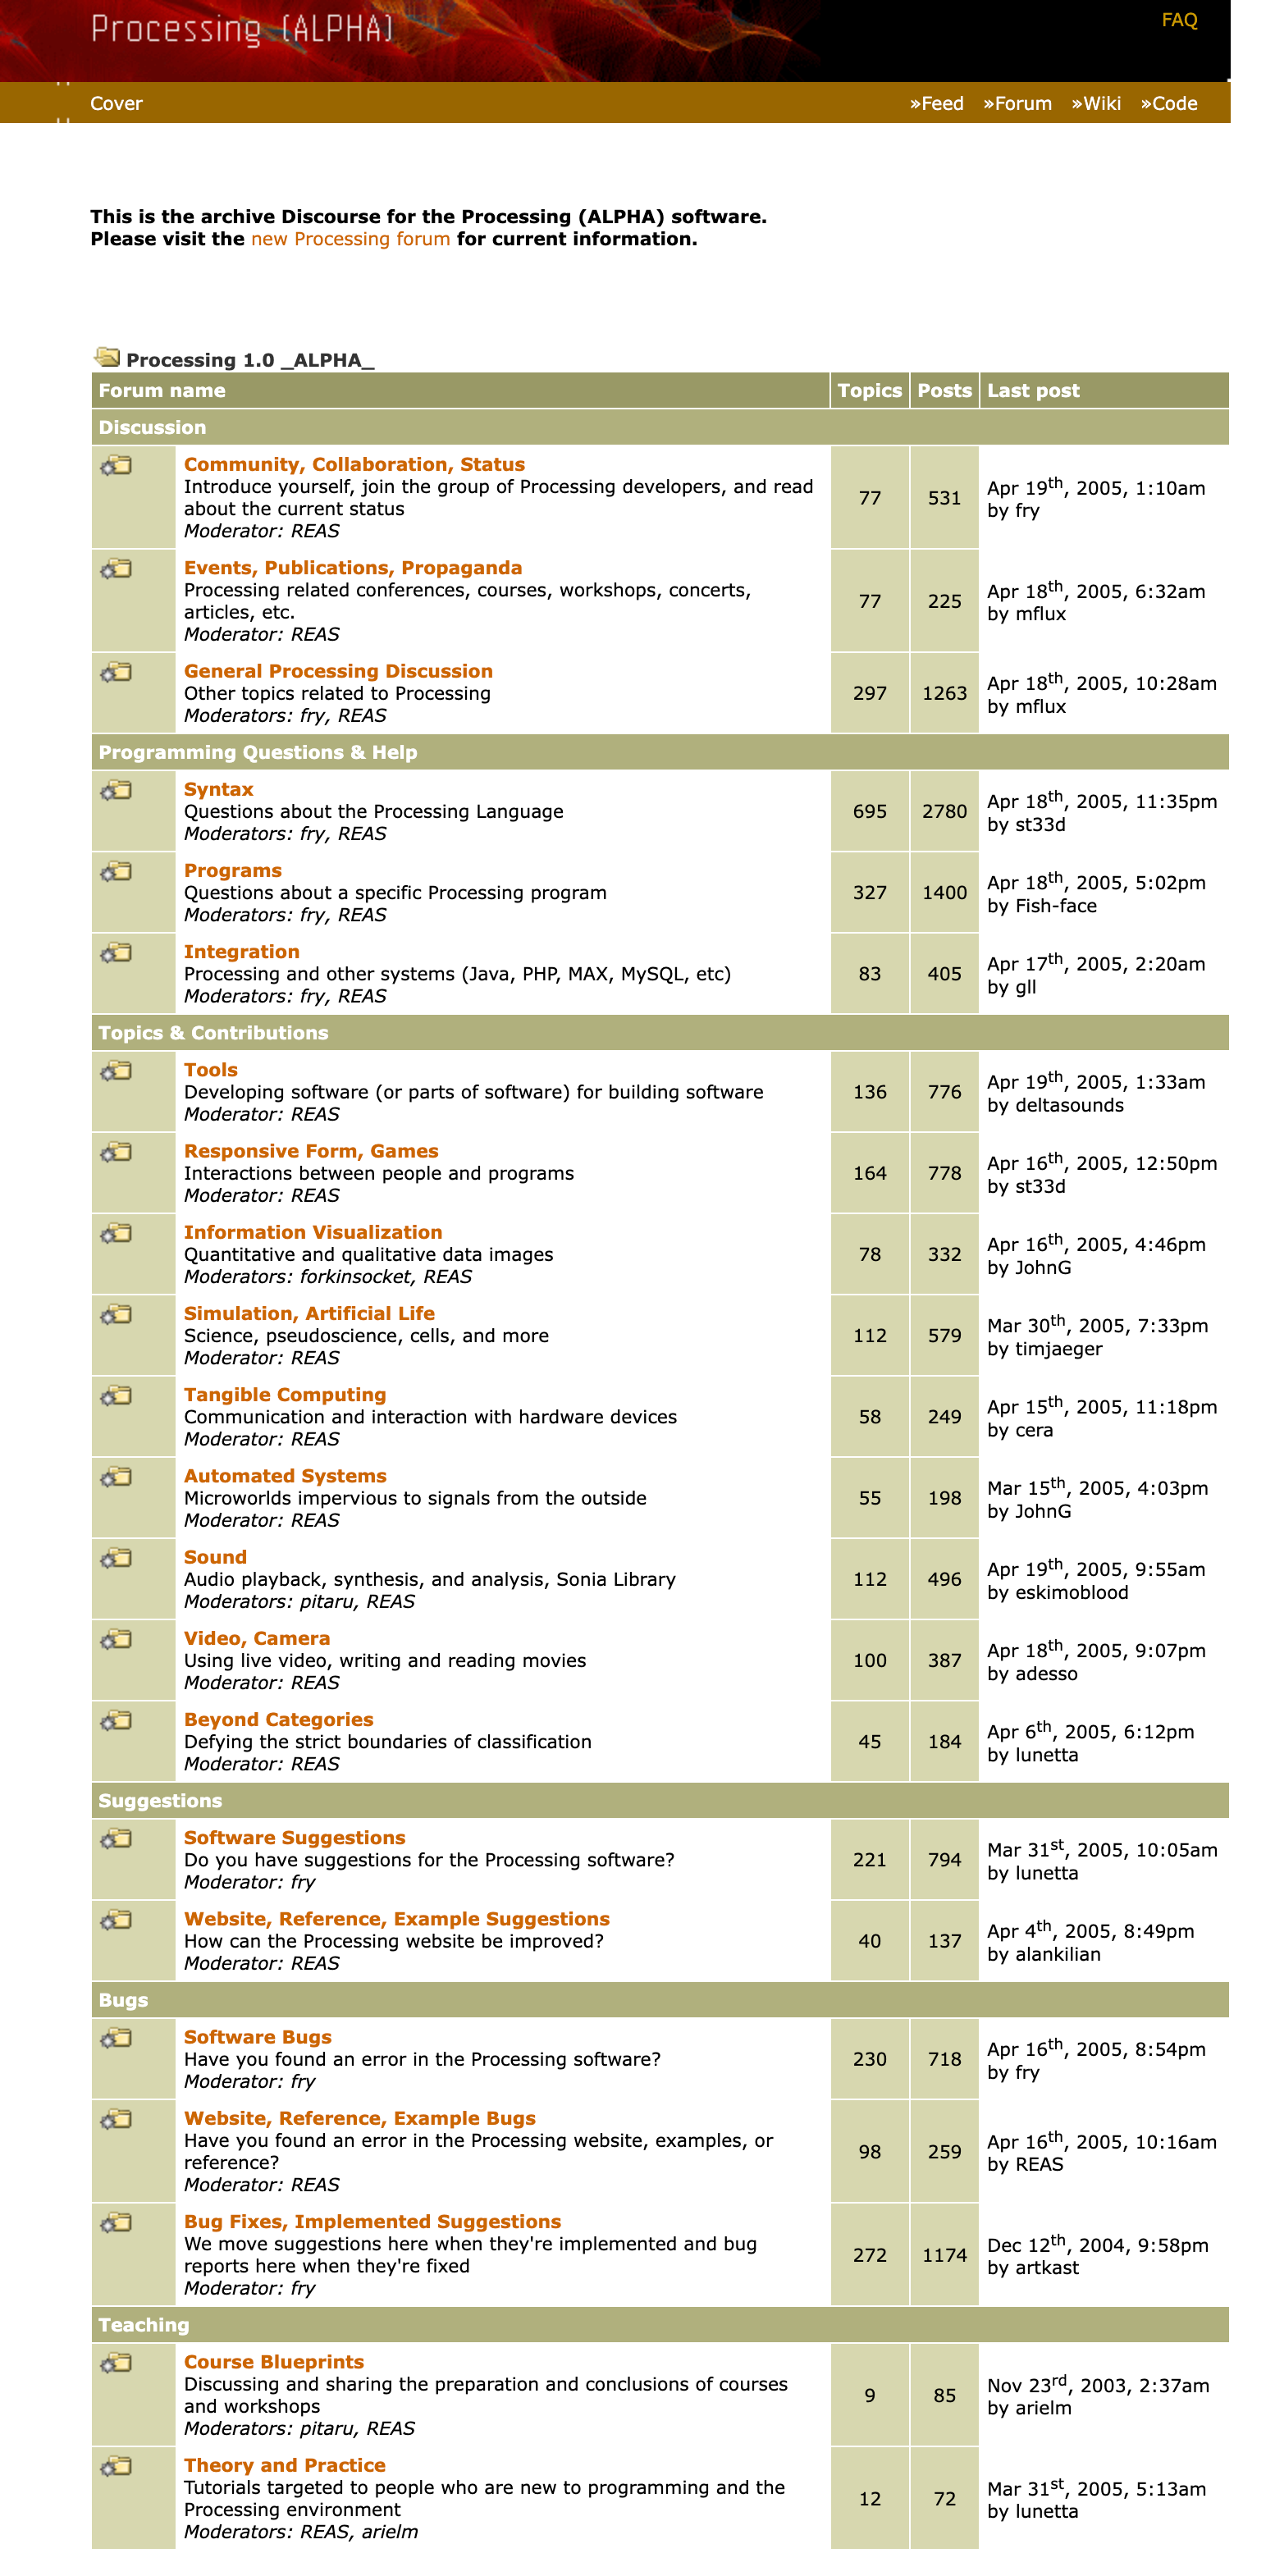
\includegraphics[width=0.7\textwidth]{images/processing_alpha_forum_screenshot.png} 
  \caption{Processing Alpha Forum (https://forum.processing.org/alpha)}
  \label{fig:alpha_forum_screenshot}
\end{figure}

\begin{figure}
  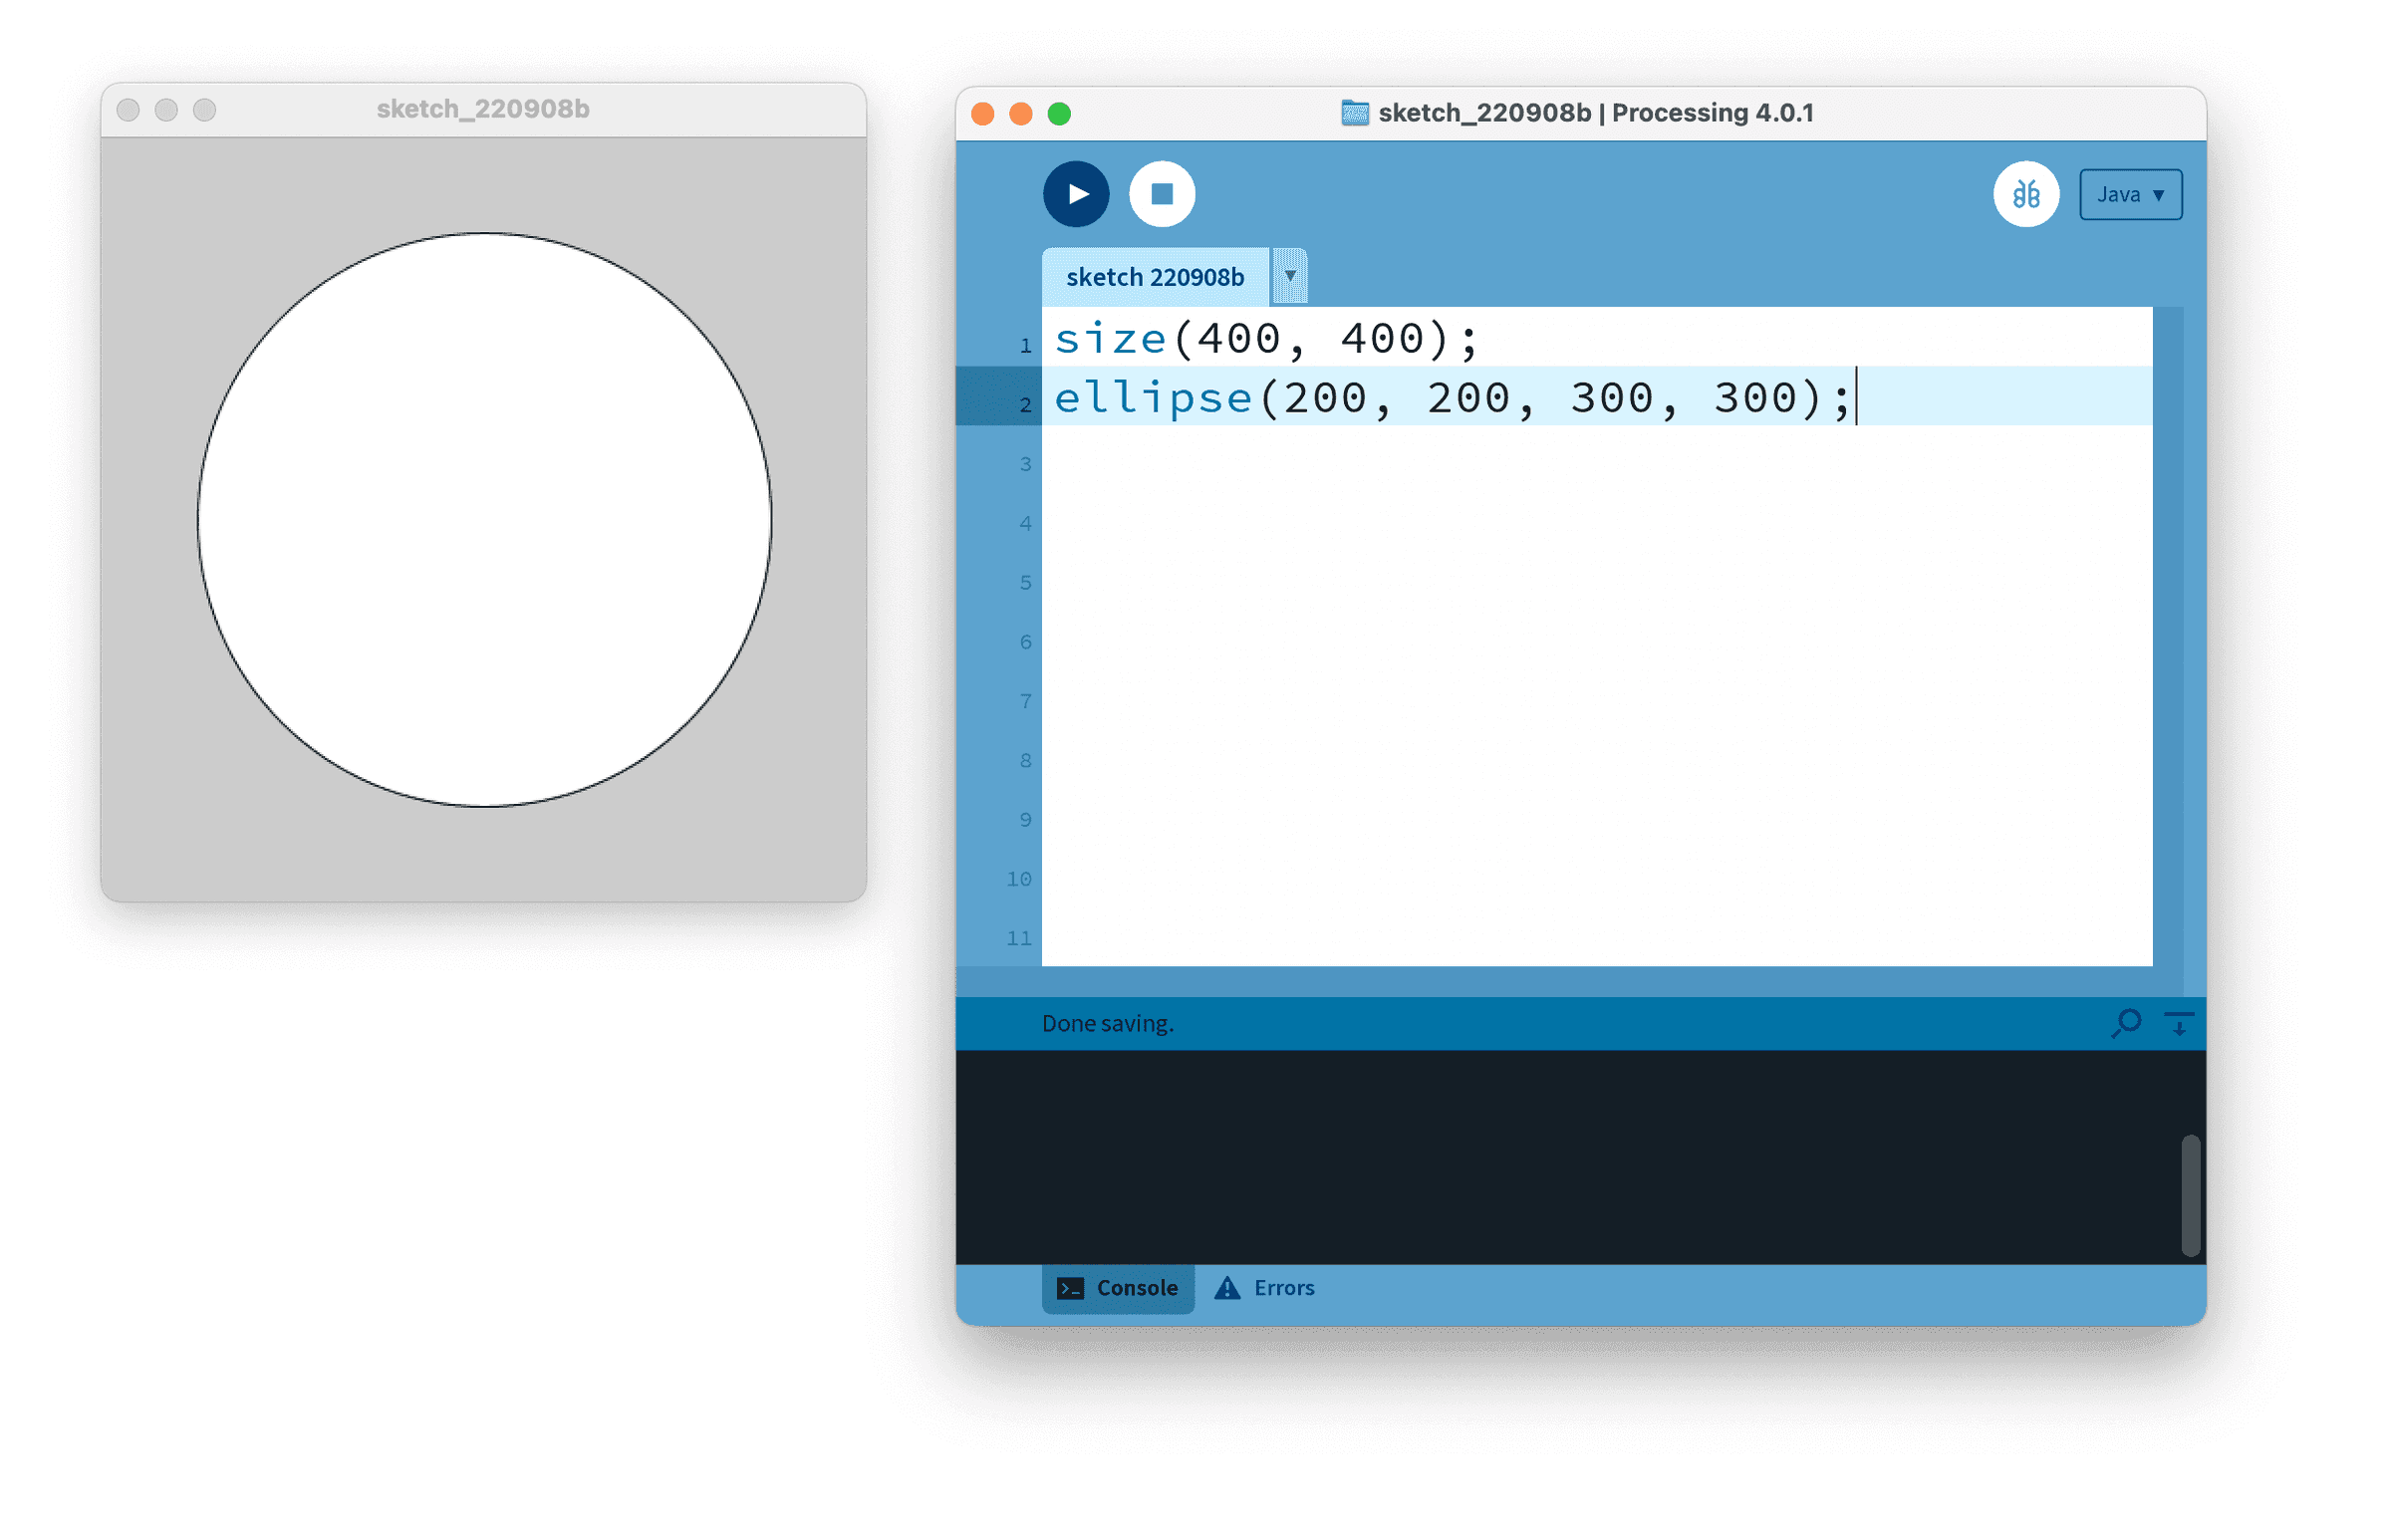
\includegraphics[width=0.5\textwidth]{images/processing_ide.png} 
  \caption{Processing IDE \parencite{reasProcessingIDE2015}}
  \label{fig:processing_ide_screenshot}
\end{figure}

% todo NN add figure about processing ide
% todo NN ne pas distinguer la litt review de l’introduction, ni la méthodo, il faudrait tout mettre dedans pour montrer (1) en quoi cela permet de formuler une question de recherche (qui reste à expliciter ici), (2) mettre en place une méthodologie pour y répondre

% todo NN Rappelle toi qu’une revue de littérature sert à préciser ton questionnement général décrcit en introduction et formuler une question de recherche puis une méthodo pour y répondre. Tu le fais heureusement déjà un peu !

% todo NN et en fin de cette grosses introduction tu pourrais mettre l’annonce du plan du mémoire, ce que vont contenir les chapitres

\section{Literature review}
\subsection{Open Source Contributions: Historical Perspective and Modern Implications}

Open source software has evolved from a grassroots, community-driven activity into a mainstream phenomenon influencing all sectors of software development. This transition has been analyzed from numerous perspectives, including Etienne Wenger's theory of Communities of Practice, which posits that learning occurs in social contexts \parencite{wengerCommunitiesPracticeLearning1998}. This theory underscores the importance of shared experiences, tools, and discourse in shaping a community's collective practice. In the context of open-source software, these dynamics offer invaluable insights into the sustainability and progression of such projects. For instance, the Processing community exemplifies more than just a collection of individual contributors; it represents a dynamic community molded by common goals and collective learning.

This communal focus contrasts sharply with the software development models described in Eric S. Raymond's seminal work "The Cathedral and the Bazaar" \parencite{CathedralBazaarMusings2002a}. The Cathedral model is marked by careful planning and centralized authority, more akin to the early GNU projects initiated by Richard Stallman in the 1980s. Conversely, the Bazaar model encourages open collaboration and decentralization—features commonly associated with contemporary open source projects. These two models can be conceptualized as endpoints of a continuum, with real-world communities of practice, like the Processing community, potentially embodying characteristics of both.

Although Richard Stallman's Free Software Movement initially utilized a Cathedral-like approach, the evolution of version control systems like Git has facilitated the adoption of more decentralized, Bazaar-like models. This technological and philosophical shift intriguingly complements Wenger's notions of "mutual engagement," "joint enterprise," and "shared repertoire"—elements that nurture a sense of community and shared objectives \parencite{wengerCommunitiesPracticeLearning1998}.

Fast-forwarding to today, the landscape now includes not just individual contributors but major corporations as well, injecting both challenges and opportunities into existing communities. The Processing project stands as a compelling case study to examine how an open-source community can preserve its foundational ethos while simultaneously adapting to contemporary requirements.

To holistically grasp the intricate interplay of social and technical factors contributing to the success of open-source initiatives, a multidimensional analysis is essential. Such an approach would synthesize various frameworks, including Wenger's Communities of Practice \parencite{wengerCommunitiesPracticeLearning1998} and Raymond's Cathedral and Bazaar models \parencite{CathedralBazaarMusings2002a}, aiming to provide a nuanced understanding of a community's past, present dynamics, and future potential.




\subsection{The Centrality of Open Source Values in Processing}

% Contextualizing the Open Source Movement
The open source movement has undeniably influenced a myriad of practical applications, ranging from operating systems like Linux to various software tools. However, its impact on the realm of creative software tools has been comparatively limited. According to Reas and Fry~\parencite[30]{reasProcessingProgrammingHandbook2007}, companies like Adobe and Microsoft largely dominate the field, limiting the open-source philosophy's penetration into the culture of arts software. % Here, you establish the broader impact of open source and point out a gap in its influence over artistic software.

% Importance of Open Source Ethos in Processing
Within this context, Processing emerges as a significant counterexample, embedding the ethos of open source at its very core. This ethos is not simply a byproduct but an intentional design choice to promote software literacy. Reas and Fry define literacy in the context of software as the ability to both "read" and "write" within a medium~\parencite[29]{reasProcessingProgrammingHandbook2007}. % This highlights how Processing intentionally incorporates open source values to facilitate a specific kind of literacy.

% Elaborating Software Literacy
In traditional print writing, literacy involves generating rhetorical tools that aim to demonstrate and convince. In contrast, computer-based literacy enables one to create processes that can simulate and decide. % This part elaborates on what software literacy entails, contrasting it with traditional forms of literacy.

% Processing's Alignment with Design Principles
Moreover, Processing exemplifies many of the Design Principles for Tools to Support Creative Thinking as suggested by Resnick~\parencite{resnickDesignPrinciplesTools}. Particularly, by fostering a culture of collaboration and open exchange, Processing does not merely align with open source motivations but elevates itself as a superior Creativity Support Tool (CST). % This wraps up the section by connecting Processing's open-source ethos to broader design principles, emphasizing its role as a potent CST.




\subsection{Understanding the Drivers of Open Source Contributions in the Processing Community}

While existing literature often focuses on the role of companies in contributing to open-source projects through complementary services like consulting, our study diverges by focusing on individual contributors. In the context of the Processing community, corporate involvement is notably lesser when compared to platforms like Linux that have substantial corporate contributions.

The 2016 Processing community survey revealed a significant number of users employ the language for educational purposes. This is consistent with Processing's design ethos, which is aimed at being educationally accessible. However, the extent to which this educational usage intersects with what can be termed as `professional use' remains unclear.

For the purpose of this study, `professional use' is understood to primarily include artists and designers. This nuanced categorization helps in probing the overlap between professional and educational use within the Processing community.

Building upon established frameworks such as the taxonomy by Bonaccorsi et al.~\cite{bonaccorsiComparingMotivationsIndividual2006}, which categorizes motivations behind open-source contributions into Economic, Social, and Technological domains, our study intends to adapt this taxonomy to suit the specific nuances of the Processing community.

\begin{figure}[h!] 
  \centering
  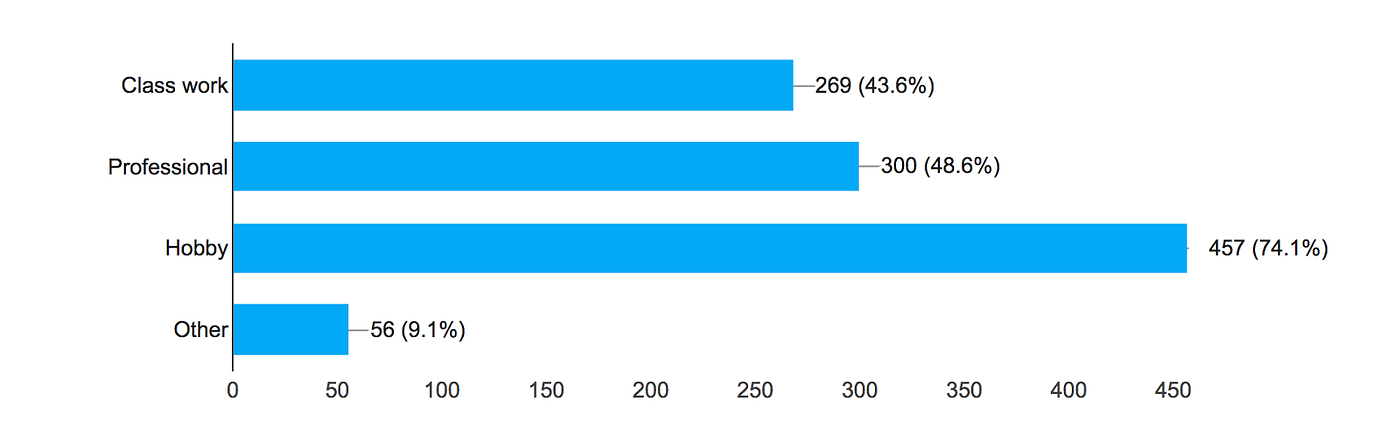
\includegraphics[width=0.9\textwidth]{images/community-survey.png} 
  \caption{Processing 2016 community survey result \parencite{2016CommunitySurvey}}
  \label{fig:community_survey}
\end{figure}

\begin{table}
    \begin{tabularx}{\textwidth}{l X} % X is a placeholder for stretching the column
    \toprule
    Motivation area & Micro level \\
    \midrule
    Economic & Monetary rewards \\
     & Low opportunity costs \\
     & Gaining a reputation among peers \\
     & Gaining future career benefits \\
    \midrule
    Social & Fun to program (Loving to code) \\
     & Altruism (gift economy) \\
     & Sense of belonging to the community \\
     & Fight against proprietary software \\
    \midrule
    Technological & Learning \\
     & Contributions and feedback from the community \\
     & Working with a bleeding-edge technology \\
     & Scratching a personal itch \\
    \bottomrule
    \end{tabularx} % End of tabularx environment
    \label{tab:taxonomy}
    \caption{Taxonomy of Individual Programmers’ Motivations. Adapted from \parencite{bonaccorsiComparingMotivationsIndividual2006}}

\end{table}

% todo NN cette taxonomie est intéressante, mais il faudrait la commenter dans le corps de texte en 2.2, qu’elle vienne nourrir ce que tu as mis au-dessus comme texte, là tu la pose rapidement sans trop détailler comment elle a été produite et ce qu’elle nous dit

%\subsection{The intersection of Creative Coding and Open Source}
%\subsection{Relevant Methodological Approaches in Computer Science and Anthropology}

\section{Methodology}

\subsection{Research Design}
Given the potential for memory bias due to the passage of time since the project's inception, this study employs a mixed-methods approach. While human memory can be fallible, introducing biases and even constructing false memories, quantitative analysis serves as a foundational component to mitigate these challenges. It allows for the identification of key contributors based on metrics such as commit frequency and significance, forum participation, and library contributions. These quantitative findings inform the selection of interviewees, acting as a preliminary filter to locate core contributors and library authors for qualitative interviews.

% todo NN attention : tu cites ici une généralité sans référence…
Anthropological studies have consistently highlighted the limitations of relying solely on quantitative data to understand the complex interplay of human experiences, beliefs, and emotions. Hence, qualitative interviews stand as a cardinal ethnographic instrument, offering access to the lived experiences, emic perspectives, and personal narratives of participants—dimensions that are often obscured in purely numerical representations.

By purposefully integrating quantitative methodologies with qualitative ethnographic approaches, this research aspires to offer a nuanced understanding of both the structural and phenomenological aspects of the Processing community.

\subsection{Quantitative Methods}
\subsubsection*{Data sources}

The research draws upon multiple data sources to form a comprehensive picture of the Processing community and its development practices. These range from forum discussions at various phases of the project to commit histories and issue trackers. The parsing status indicates the extent to which each data source has been prepared for analysis. 
\begin{table}[h]
    \raggedright
    \caption{Data sources}
    \label{table:data-sources}
    \begin{tabular}{l l l c}
        \toprule
        Name & Type & Status \\
        \midrule
        Processing alpha forum & Forum & Parsed \\
        Processing beta forum & Forum & Parsed  \\
        Processing 1.0 forum & Forum & Downloaded \\
        Processing 2.0 and 3.0 forum & Forum  & Not downloaded \\
        Current processing forum & Forum & Not downloaded\\
        Github project & Commit history & Parsed \\
        Processing Release Data & Release notes & Parsed \\
        Github Release Data & Release notes \& download statistics & Parsed \\
        Processing libraries\textsuperscript{*} & Software release information & Parsed \\

        \bottomrule
        \multicolumn{3}{l}{\footnotesize \textsuperscript{*}Note: The data set was reconstructed from the processing website archive and is not complete.}
    \end{tabular}
  \end{table}        

\subsubsection*{Evolution of Community Discussion Platforms}
In the early days of the Processing project, community interactions predominantly took place on forums. These forums served as a primary channel for users to share experiences, discuss problems, and seek help. Notably, the forum discussions underwent significant transformations in terms of platforms over the years, as can be observed in Table \ref{table:forums}. \parencite{ProcessingForum}

\begin{table}[h]
    \raggedright
    \caption{Archival forums composition}
    \label{table:forums}
    \begin{tabular}{l l l c}
        \toprule
        Forum name & Years & URL \\
        \midrule
        Processing alpha forum & 2002-2005 & \href{https://forum.processing.org/alpha/}{forum.processing.org/alpha} \\
        Processing beta forum & 2005-2010 & \href{https://forum.processing.org/beta/}{forum.processing.org/beta}  \\
        Processing 1.0 forum & 2010-2013 & \href{https://forum.processing.org/one/}{forum.processing.org/one} \\
        Processing 2.0 and 3.0 forum & 2013-2018 & \href{https://forum.processing.org/two/}{forum.processing.org/two} \\
        Current processing forum & 2018 - now & \href{https://discourse.processing.org/}{discourse.processing.org} \\
        \bottomrule
    \end{tabular}
  \end{table}

This dynamic shift from one platform to another indicates an evolving user-base and a growing set of needs and tools that community members require for effective collaboration.

\subsubsection*{Shift in Software-Related Discussions}

Initially, software-related discussions were confined to these forums. However, as the project matured, the complexity of issues warranted more specialized platforms for effective tracking and resolution. Consequently, the community transitioned from forums to Bugzilla \parencite{BugzillaArchiveProcessing} and eventually to GitHub Issues\parencite{ProcessingProcessingSource}\parencite{ProcessingProcessing4Processing}. 

\subsubsection*{The Ecosystem of Libraries}
An important milestone in the Processing ecosystem was the introduction of libraries. These libraries extended the functionalities of the base platform, thereby attracting a broader range of users and contributors. Such an analysis not only sheds light on the diversification of the project but also identifies key contributors and library authors who could potentially be sought out for qualitative interviews. The identification of these contributors adds another layer to our understanding of community participation.

\begin{figure}[h!] 
    \centering 
    \includesvg[pretex=\sffamily\fontsize{5.58pt}{8pt}\selectfont, width=1\textwidth, keepaspectratio]{images/figure-libraries.svg}
    \caption{Distribution of Libraries in the Processing Project}
    \label{figure:libraries}  
  \end{figure}

% todo NN ce serait bien de mieux valoriser cette figure 2 visuellement, dans une mise en page aérée et large


% todo add
%\subsubsection{Forum Textual Analysis: Approach and Tools}
%The research process began by manually reading the forum to identify themes and complemented with quantitative approaches. 
%todo forum composition





% \begin{figure}[h] 
%   \centering 
%   \includegraphics[width=1\textwidth]{} 
%   \caption[Ben Fry at PCD 2018]{Ben Fry with conference attendees. Source: \citefield{guptaBenFryConference2018}{author}, Medium, \citeyear{guptaBenFryConference2018}.}

%   \label{figure:benfry-pcd}  
% \end{figure}
% \textbf{Note.} Source: \textcite{guptaBenFryConference2018}.

\subsection{Qualitative Methods}
\begin{figure}[H]
  \begin{minipage}{\textwidth}
    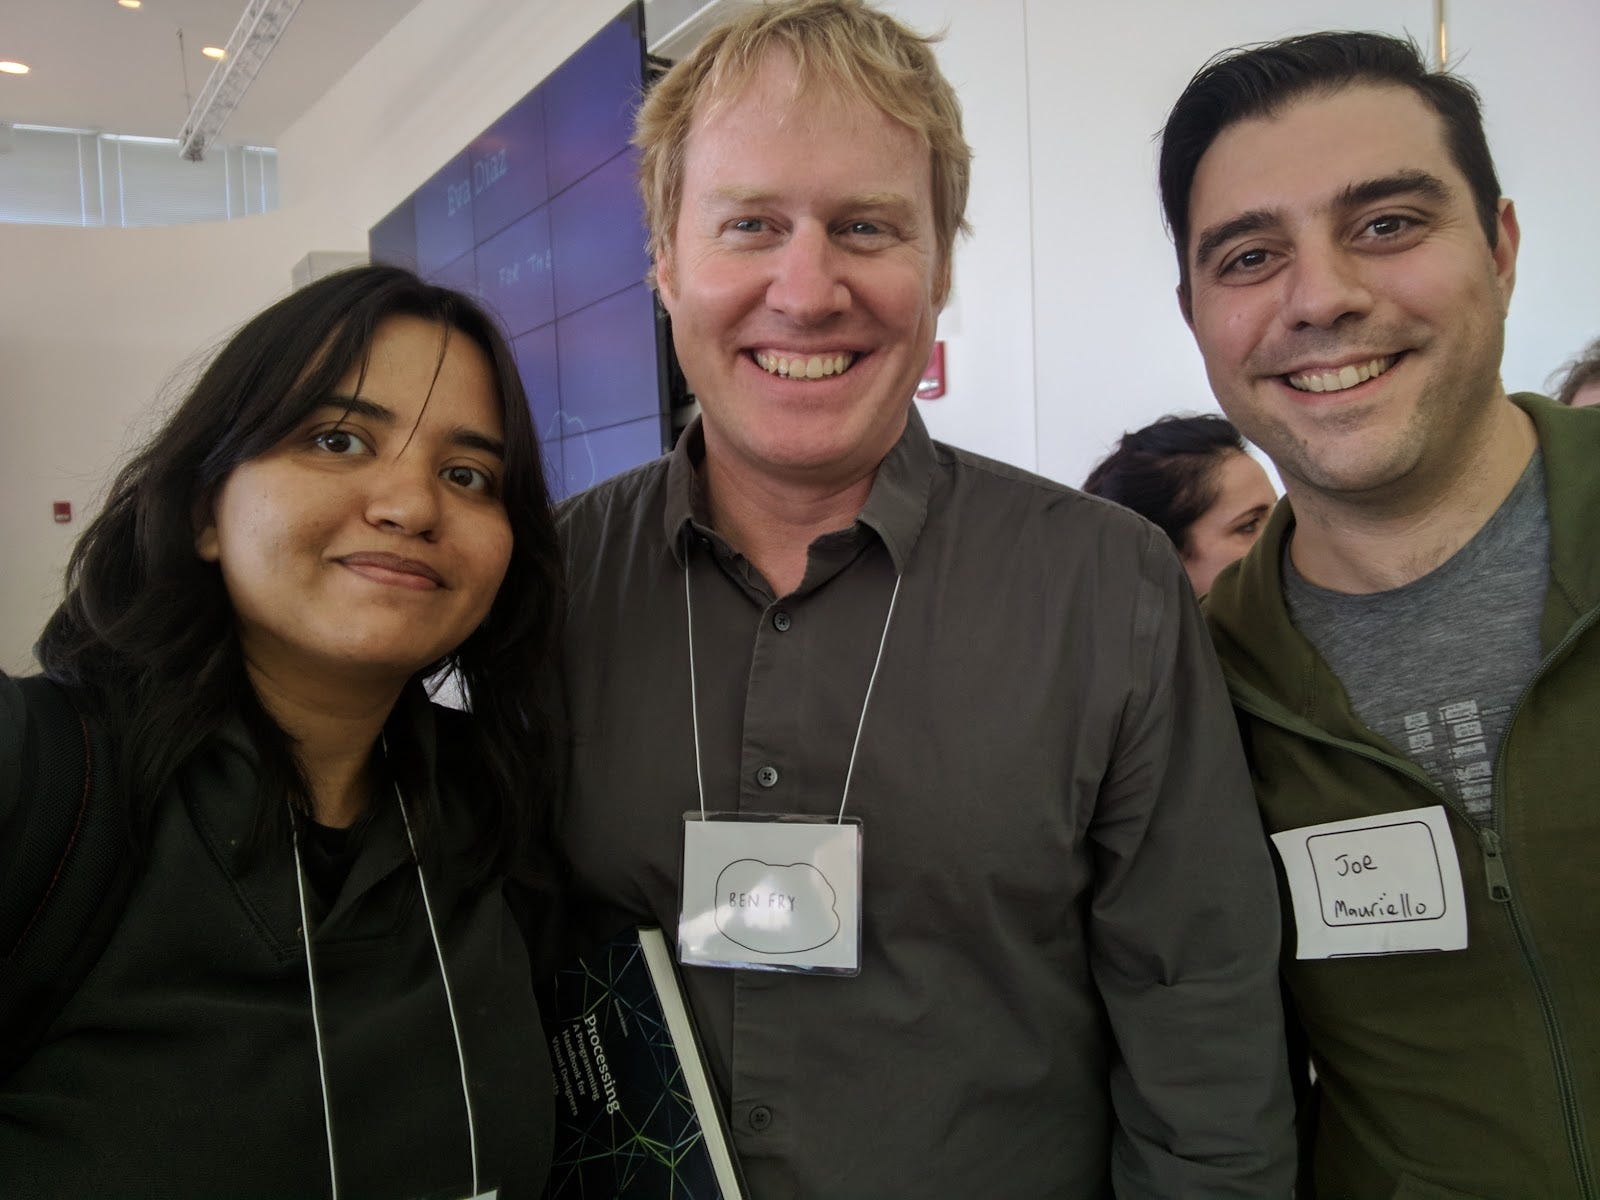
\includegraphics[width=\linewidth]{images/pcd2018.jpg}
    \caption[Ben Fry at PCD 2018]{Ben Fry with conference atendees at Processing Community Day 2018. \fullcitefigure{guptaBenFryConference2018}.}
    \label{fig:benFry}
    
  \end{minipage}
\end{figure}

For this study, the primary qualitative method utilized is semi-structured interviews. This choice was driven by the need for a flexible yet organized approach to gather in-depth insights from participants.

The selection of interviewees was strategically informed by the results of quantitative analyses, particularly in areas where abundant data was available. This methodological triangulation enhances the reliability and depth of the findings.

Interviewees were mainly categorized into distinct populations, which are as follows:

\begin{itemize}
    \item Individuals with the highest number of git commits during the period of the alpha forum, from August 2, 2002, to April 19, 2005.
    \item Members who exhibited the most significant activity on the alpha forum within the same time frame.
    \item Authors of libraries with the most frequent release activity, based on available data spanning from October 26, 2011, to June 8, 2014.
\end{itemize}

Although the Processing Foundation was formalized subsequent to the period under study, it was deemed necessary to include its founding board members in the pool of interviewees. The foundation project’s mission started as the promotion of software and visual literacy through making the development of the core API, and Processing Development Environment (PDE) sustainable. Therefore, its influence is integral to the present investigation.\parencite{robertsProcessingFoundationForm2013}

There are also noteworthy contributors to the Processing ecosystem that fall outside the scope of this paper. These include:

\begin{itemize}
    \item Individuals engaged in writing documentation, examples, and books.
    \item Those participating in or organizing local Processing Community Days or other community events.
    \item Google Summer of Code participants and mentors.
    \item Recipients of fellowship programs.
\end{itemize}

\subsection{The Role of the Processing Foundation}

The Processing Foundation was established in 2012 by Casey Reas, Ben Fry, and Daniel Shiffman with the primary objective of sustaining the software's development and broadening its reach. According to Fry and Reas, ``The vast majority of the code is written by the same small number of people volunteering their time — there are no paid full-time developers'' \parencite[p.~13]{fryModernPrometheusHistory2018}.

\begin{figure}[h]
    \centering
    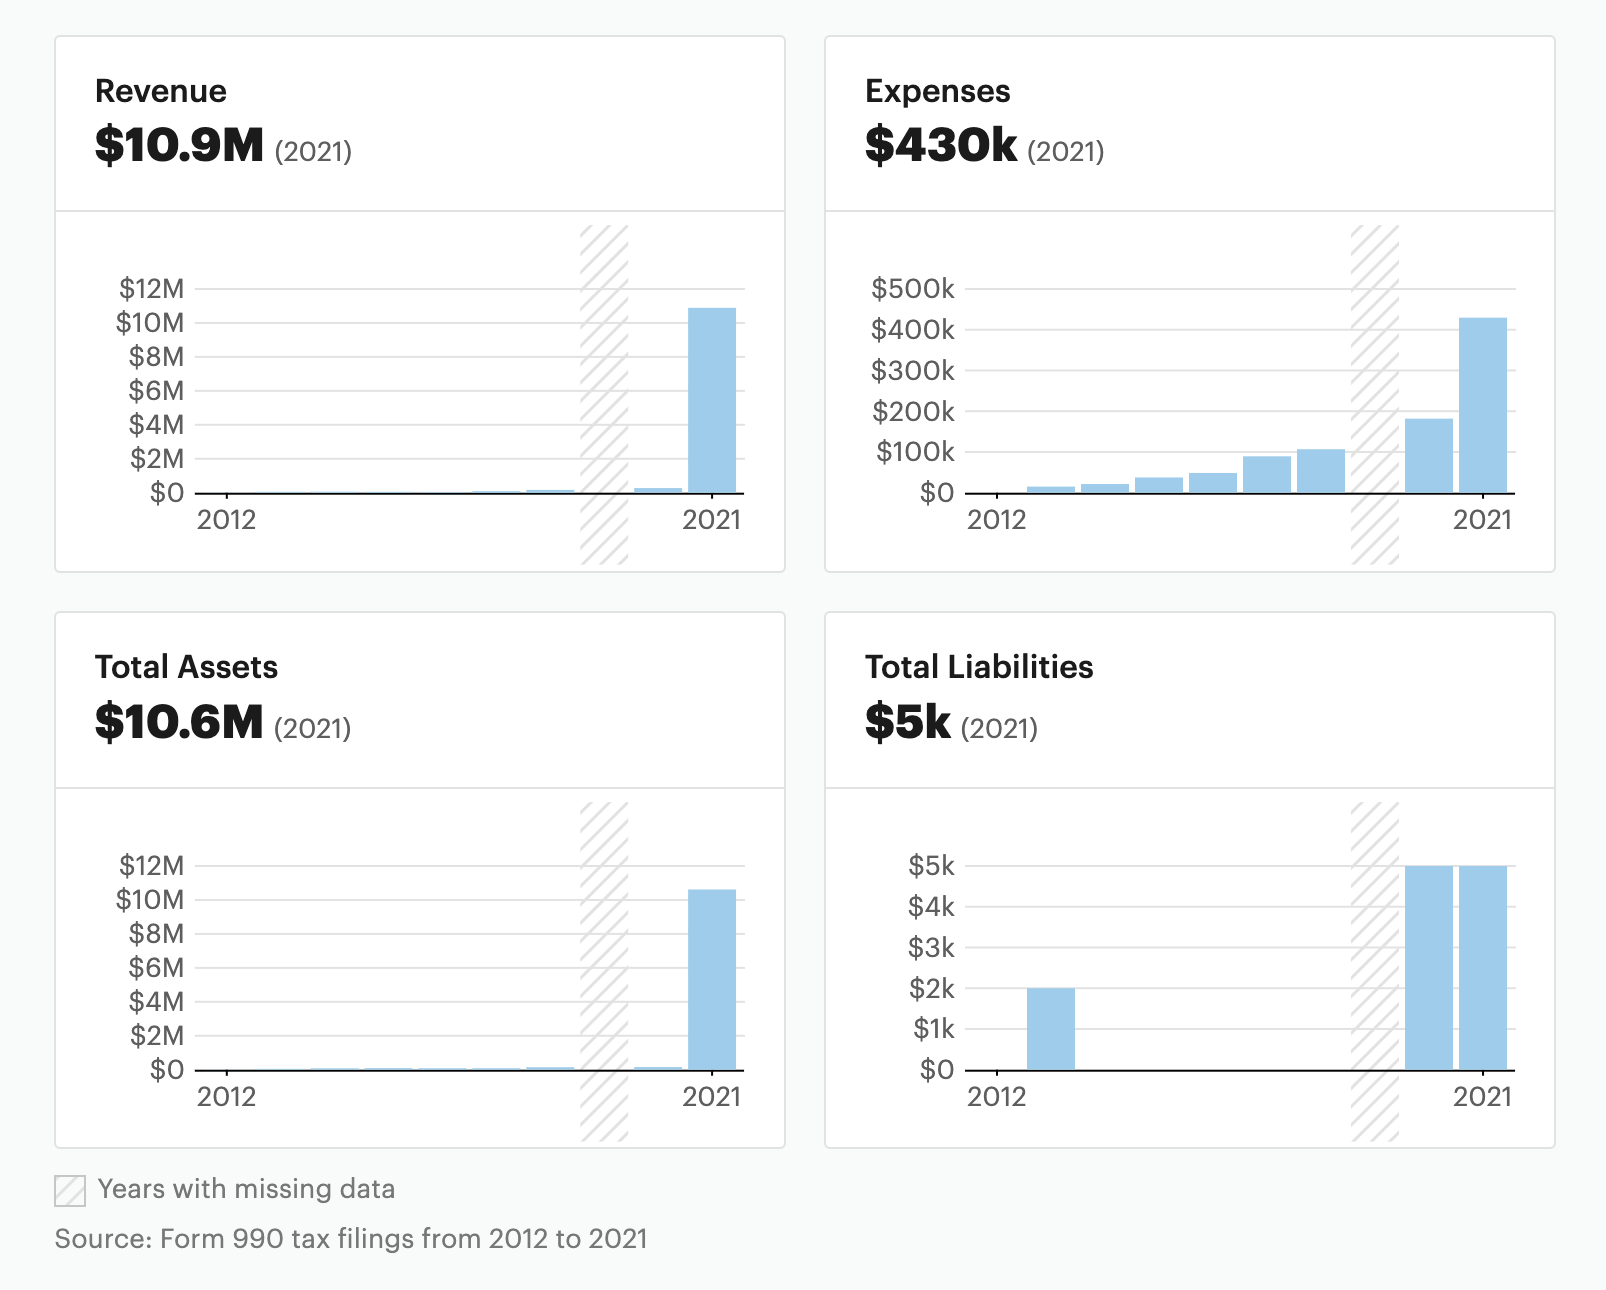
\includegraphics[width=0.9\textwidth]{images/foundation-finances.png} 
    \caption{Financial growth of the Processing Foundation over the years Source: \parencite{ProcessingFoundationNonprofit2013}}
    \label{fig:foundation-finances}
\end{figure}

As shown in Figure~\ref{fig:foundation-finances}, the foundation's revenue has experienced modest growth, increasing from \$11,235 to \$273,520. Remarkably, it reached a peak revenue of \$10,889,998 in the fiscal year 2021. Throughout its history, the principal source of funding for the foundation has predominantly come from contributions. 

However, the allocation of these funds has been a point of contention within the organization. Most notably, a public disagreement in 2023 led to the resignation of Ben Fry, a long-standing board member and contributor. It should be noted that Fry's perspective on the matter was not universally accepted among the foundation's other founding members. \parencite{benfry[@ben_fry]HaveMadeExtremely2023} \parencite{caseyreas[@reas]EarlierThisWeek2023} \parencite{danielshiffman[@shiffman]WouldPostNote2023}

\section{Data Presentation and Analysis}

\subsection{Quantitative Findings}

\subsection{Release early, release often}

The maxim "Release early, release often," attributed to Eric S. Raymond in his seminal text "The Cathedral and the Bazaar" \parencite{raymondCathedralBazaar1999}, is often touted as a catalyst for vibrant open-source communities. In particular, projects like Linux have benefited from this approach, allowing rapid integration of contributions from a distributed network of contributors. This not only boosts the morale of individual contributors but also creates a dynamic and responsive development environment.

However, the Processing project presents a departure from this pattern. The time-between-releases data, presented in the table below, reveals periods of intense activity interlaced with long intervals of inactivity, complicating a straightforward mapping onto the “Release early, release often” model.

\begin{tabular}{ll}
  \toprule
   & time\_between\_releases \\
  \midrule
  count & 60 \\
  mean & 20 days 15:11 \\
  std & 47 days 00:10 \\
  min & 0 days 00:00 \\
  25\% & 1 days 00:00 \\
  50\% & 3 days 00:00 \\
  75\% & 26 days 18:00 \\
  max & 338 days 00:00 \\
  \bottomrule
\end{tabular}

Note: Early releases do not have timestamps, and some releases occur on the same day, making statistical interpretation less straightforward.

\begin{figure}[h!] 
  \centering
  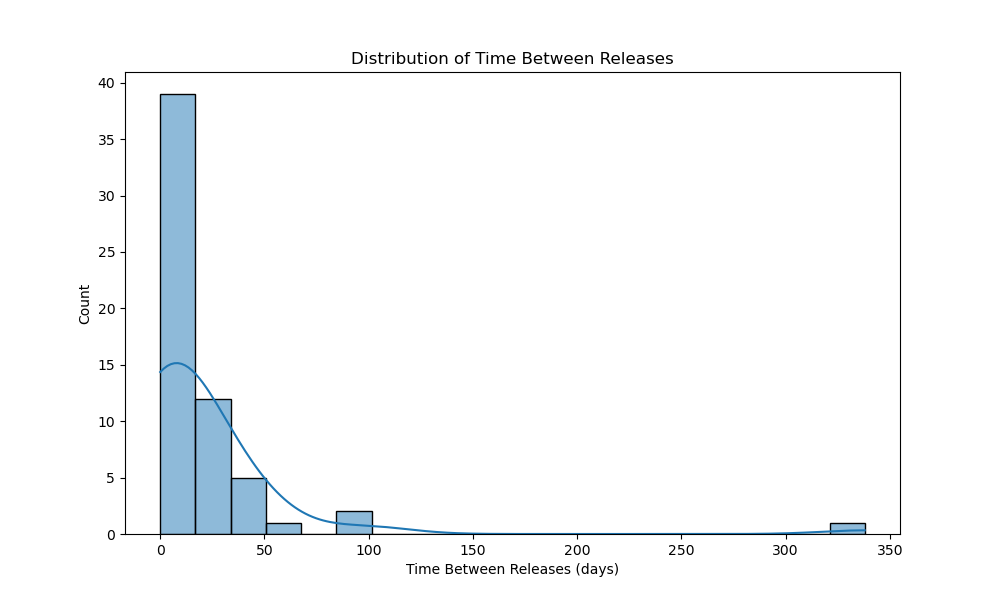
\includegraphics[width=0.9\textwidth]{images/time_between_releases_histogram.png} 
  \caption{Time between releases histogram}
  \label{fig:releases_frequency_histogram}
\end{figure}

\begin{figure}[h!] 
  \centering
  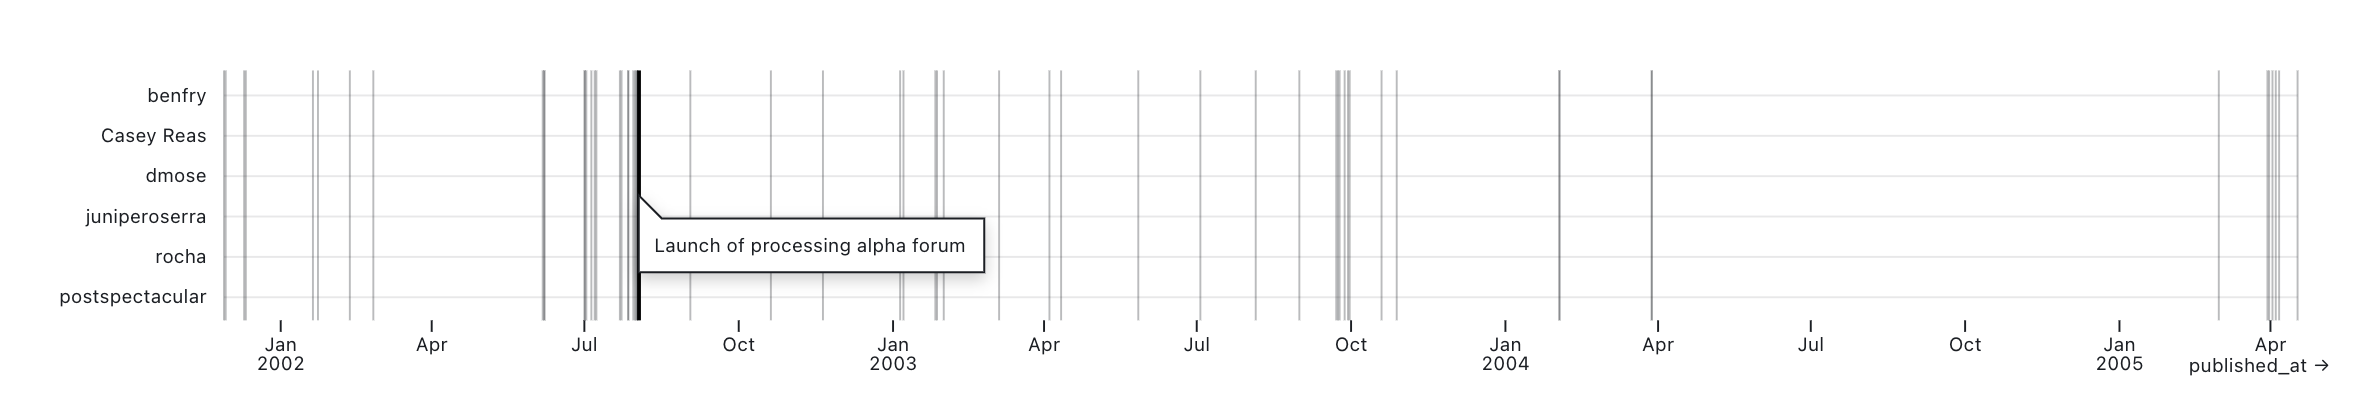
\includegraphics[width=0.9\textwidth]{images/releases-lines.png} 
  \caption{Time between releases}
  \label{fig:releases-lines}
\end{figure}

What makes Processing a particularly interesting case is that, contrary to what one might expect from Raymond's model, most contributions appear to be made by a centralized figure—Ben Fry, the project's main architect—rather than a broad community of external contributors. This effectively shifts the project's development model closer to a cathedral-like structure for core components, as reflected by Ben's direct control over major releases. 

Moreover, the project’s side-project nature is confirmed by revision comments such as one from 05/01/2003, which reads: "hopefully January 2003 will be a good month for p5, as I have a short bit of time to work on it [...] I hope to get a few revisions out this month so I can get back to my 'real' work." These comments illuminate that, for core contributors, Processing is not necessarily viewed as a full-time commitment.

The perception of Processing as a side project rather than a full-time commitment for its core contributors is corroborated through multiple channels. For example, a revision comment from May 1, 2003, highlights this sentiment, stating, ``hopefully January 2003 will be a good month for p5, as I have a short bit of time to work on it [...] I hope to get a few revisions out this month so I can get back to my `real' work.'' This observation is further substantiated by a 2021 study titled ``Graphic design in the post-digital age: a survey of practices fueled by creative coding,'' which notes that Processing began as a personal initiative and was largely developed during nights and weekends. The study further reveals that the project received indirect funding from MIT through Fry's graduate stipend, and from IDII through Reas's salary, again indicating its ancillary nature in the professional lives of its principal contributors~\parencite[396]{conradGraphicDesignPostdigital2021}.

It is worth noting that the logistics of releasing software were more complex in the early 2000s than they are today. As can be seen in Figure~\ref{fig:processing-cd} of a mini CD from October 2002 illustrates, distributing software was not as straightforward as pushing updates to a Git repository.

\begin{figure}[h!] 
  \centering
  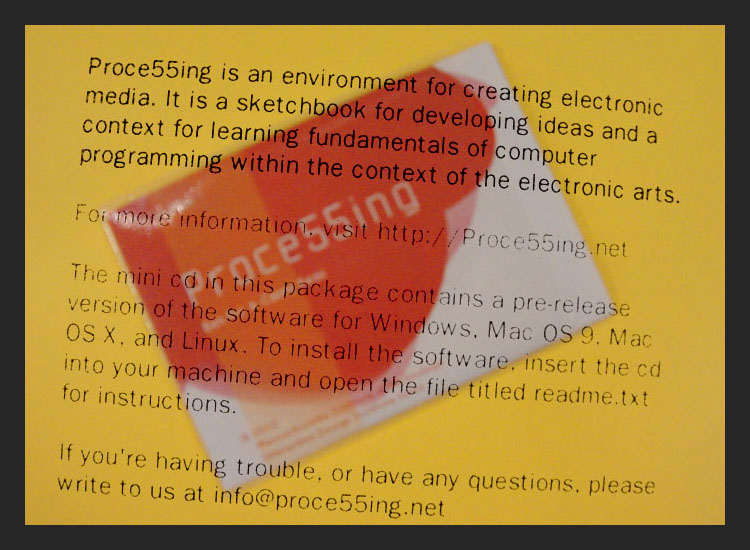
\includegraphics[width=0.9\textwidth]{images/processing-mini-cd.jpg} 
  \caption{MINI CDs CREATED FOR SPONSORS at the MEDIA LAB OPEN HOUSE october 2002}
  \label{fig:processing-cd}
\end{figure}

\subsubsection{Trends in Git Commits}

The \textit{Processing} project illuminates a crucial challenge often faced by open source communities: the dependency on key contributors. In the case of Processing, Ben Fry's central role over the past two decades raises concerns about the project's resilience and sustainability. His substantial contributions create a high-risk situation termed the "bus factor" \parencite{BusFactor2023}, which indicates how vulnerable a project becomes when overly reliant on a single or a small number of contributors. This vulnerability is not unique to Processing, as such dependency models are commonly observed across open source projects, often humorously discussed in popular culture \parencite{munroeDependency2020}.

The imbalanced contribution landscape is vividly illustrated in Figure~\ref{fig:alpha-commits}. During the period of the alpha forum, only six individuals contributed code to the repository. This stands in stark contrast to the activity on the forum, where over 1000 individuals were engaged in discussions and queries. The commits themselves were also sporadic and infrequent. As Casey aptly points out: ``I think one thing that’s important to clarify is that Ben Fry, my collaborator, is the primary software engineer of the project [...]'' \parencite[p. 330]{conradGraphicDesignPostdigital2021}.

\begin{figure}[h!] 
  \centering 
  \includesvg[pretex=\sffamily\fontsize{5.58pt}{8pt}\selectfont, width=1\textwidth, keepaspectratio]{images/processing-alpha-commits.svg}
  \caption{Commits up to and including the Processing alpha forum}
  \label{fig:alpha-commits}  
\end{figure}

This discrepancy between the number of code contributors and forum participants is indeed profound, as corroborated by the subsequent visualizations ~\ref{fig:top12-github} and comic anecdotes ~\ref{fig:dependency_comic}. The limited number of contributors to the codebase and the concentrated responsibility on a few individuals amplify the bus factor risk, an issue that warrants deeper investigation and consideration for the long-term health of the project.


\begin{figure}[h!] 
    \centering 
    \includesvg[pretex=\sffamily\fontsize{5.58pt}{8pt}\selectfont, width=1\textwidth, keepaspectratio]{images/figure-top12-github.svg}
    \caption{Top 12 source code contributors by number of commits}
    \label{fig:top12-github}  
  \end{figure}

\begin{figure}[h!] 
    \centering
    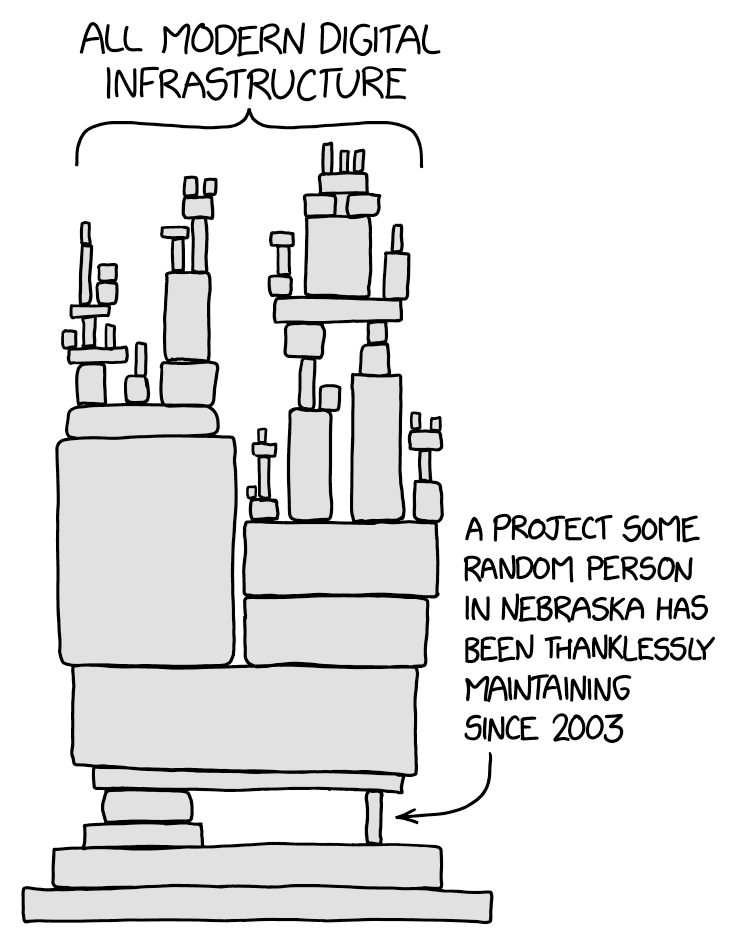
\includegraphics[width=0.5\textwidth]{dependency.png} 
    \caption{Dependency}
    \label{fig:dependency_comic}
    \small Source: \textit{XKCD}, \url{https://xkcd.com/2347/}, licensed under CC BY-NC 2.5.
\end{figure}

% \subsubsection{Patterns in Forum Contributions}

% Although Ben Fry remains the most active contributor in forum discussions, the activity distribution is more balanced compared to Git commits. This may be due to the broader range of topics discussed, including technical issues and bugs.
% A total of 1039 people posted on the forum in that time period. There were core people there that were actively participating as can be seen in the ~ref{processing-alpha-dot}

% Casey Reas “I would say that the period from around 2002 to 2006 was one when it felt almost like a unified international community created around the forum.” ([“Graphic design in the post-digital age: a survey of practices fueled by creative coding”, 2021, p. 331](zotero://select/library/items/GKA2GIS5)) ([pdf](zotero://open-pdf/library/items/QL4IRL3M?page=333&annotation=BRCSCF56))

% \begin{figure}[h!] 
%   \centering
%   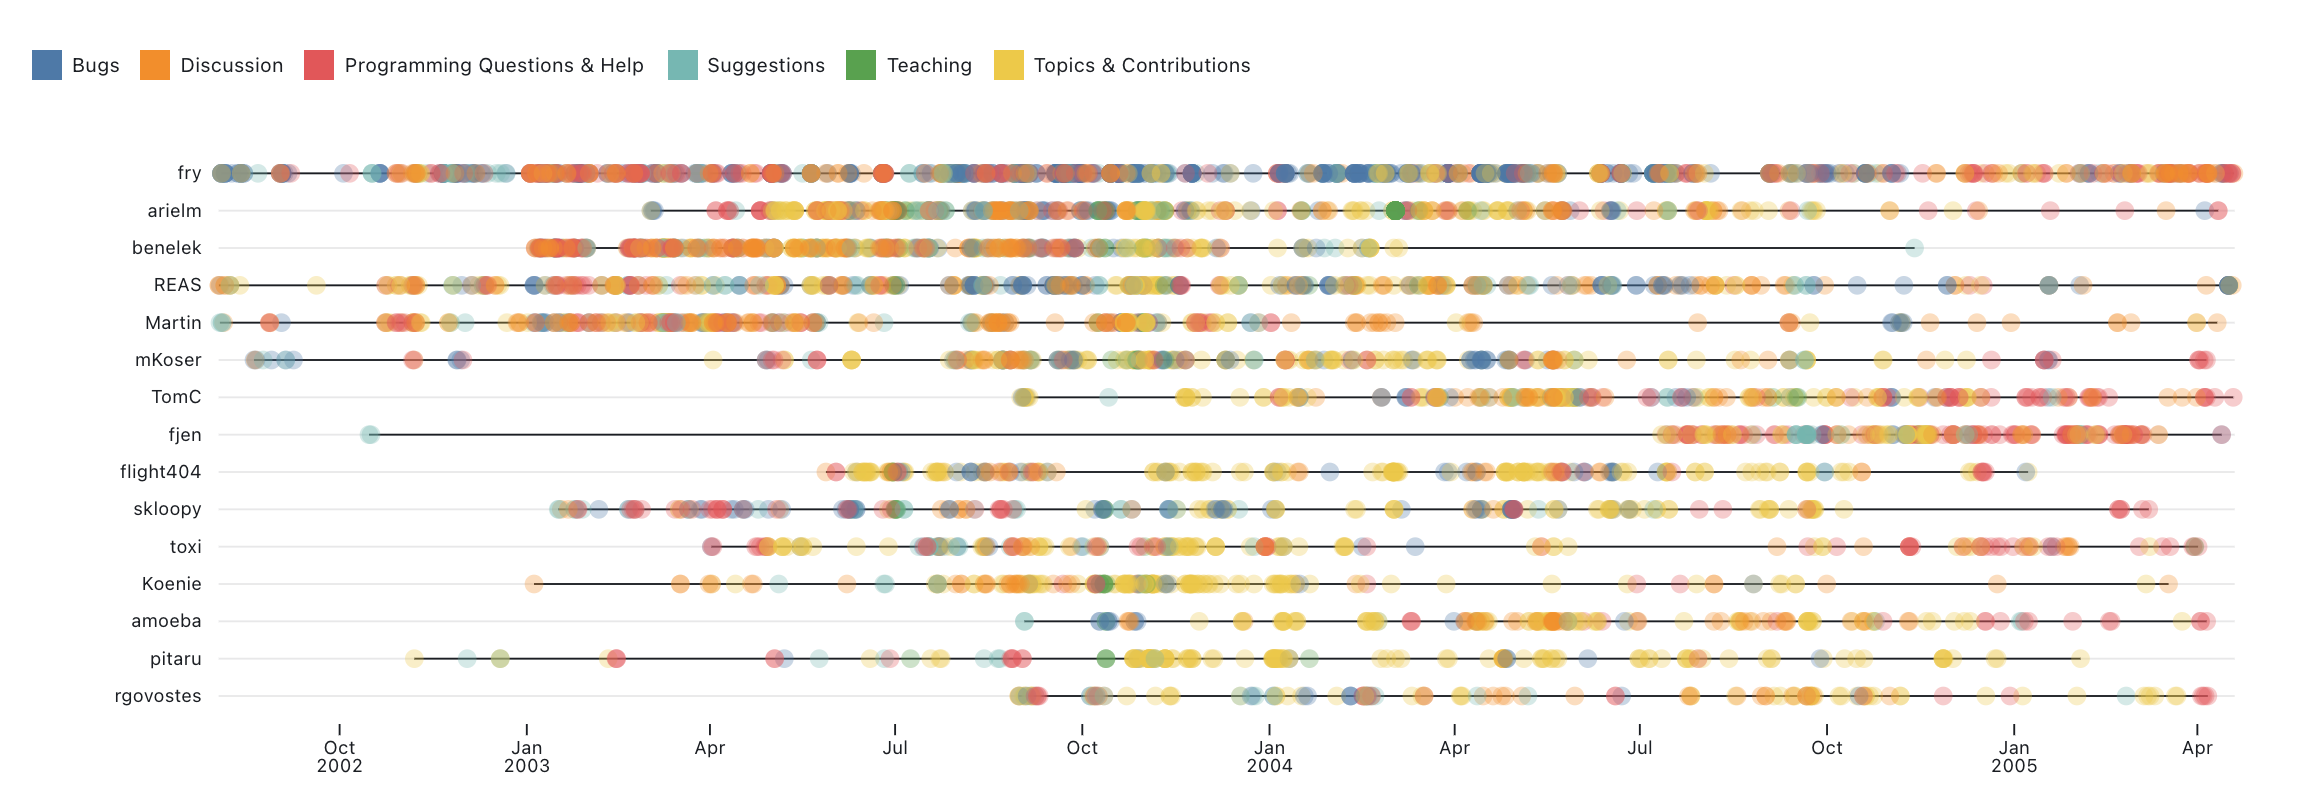
\includegraphics[width=0.9\textwidth]{images/alpha-forum-top15.png} 
%   \caption{Posting of 15 most active contributors on the alpha forum}
%   \label{fig:processing-alpha-dot}
% \end{figure}

% “"Given enough eyeballs, all bugs are shallow." I dub this: "Linus's Law."” ([Raymond, 1999, p. 29](zotero://select/library/items/87U5FDLI)) ([pdf](zotero://open-pdf/library/items/UZP875I7?page=7&annotation=89BX42PF))
% While this didn't translate well to the number of code contributors, we can see an incresed activity in the forum adjacent to releases suggesting that people contribute to at least finding bugs as seen in ~ref{figure:forum-git-activity}

\subsubsection{Patterns in Forum Contributions}

Ben Fry is the most active forum contributor, but the activity distribution is more balanced than in Git commits, possibly due to the diverse topics covered, including technical queries and bugs. A total of 1,039 individuals contributed to the forum discussions as shown in Figure~\ref{fig:processing-alpha-dot}.

Casey Reas suggests that from 2002 to 2006, the forum cultivated a "unified international community" \parencite[331]{conradGraphicDesignPostdigital2021}. 

\begin{figure}[h!]
  \centering
  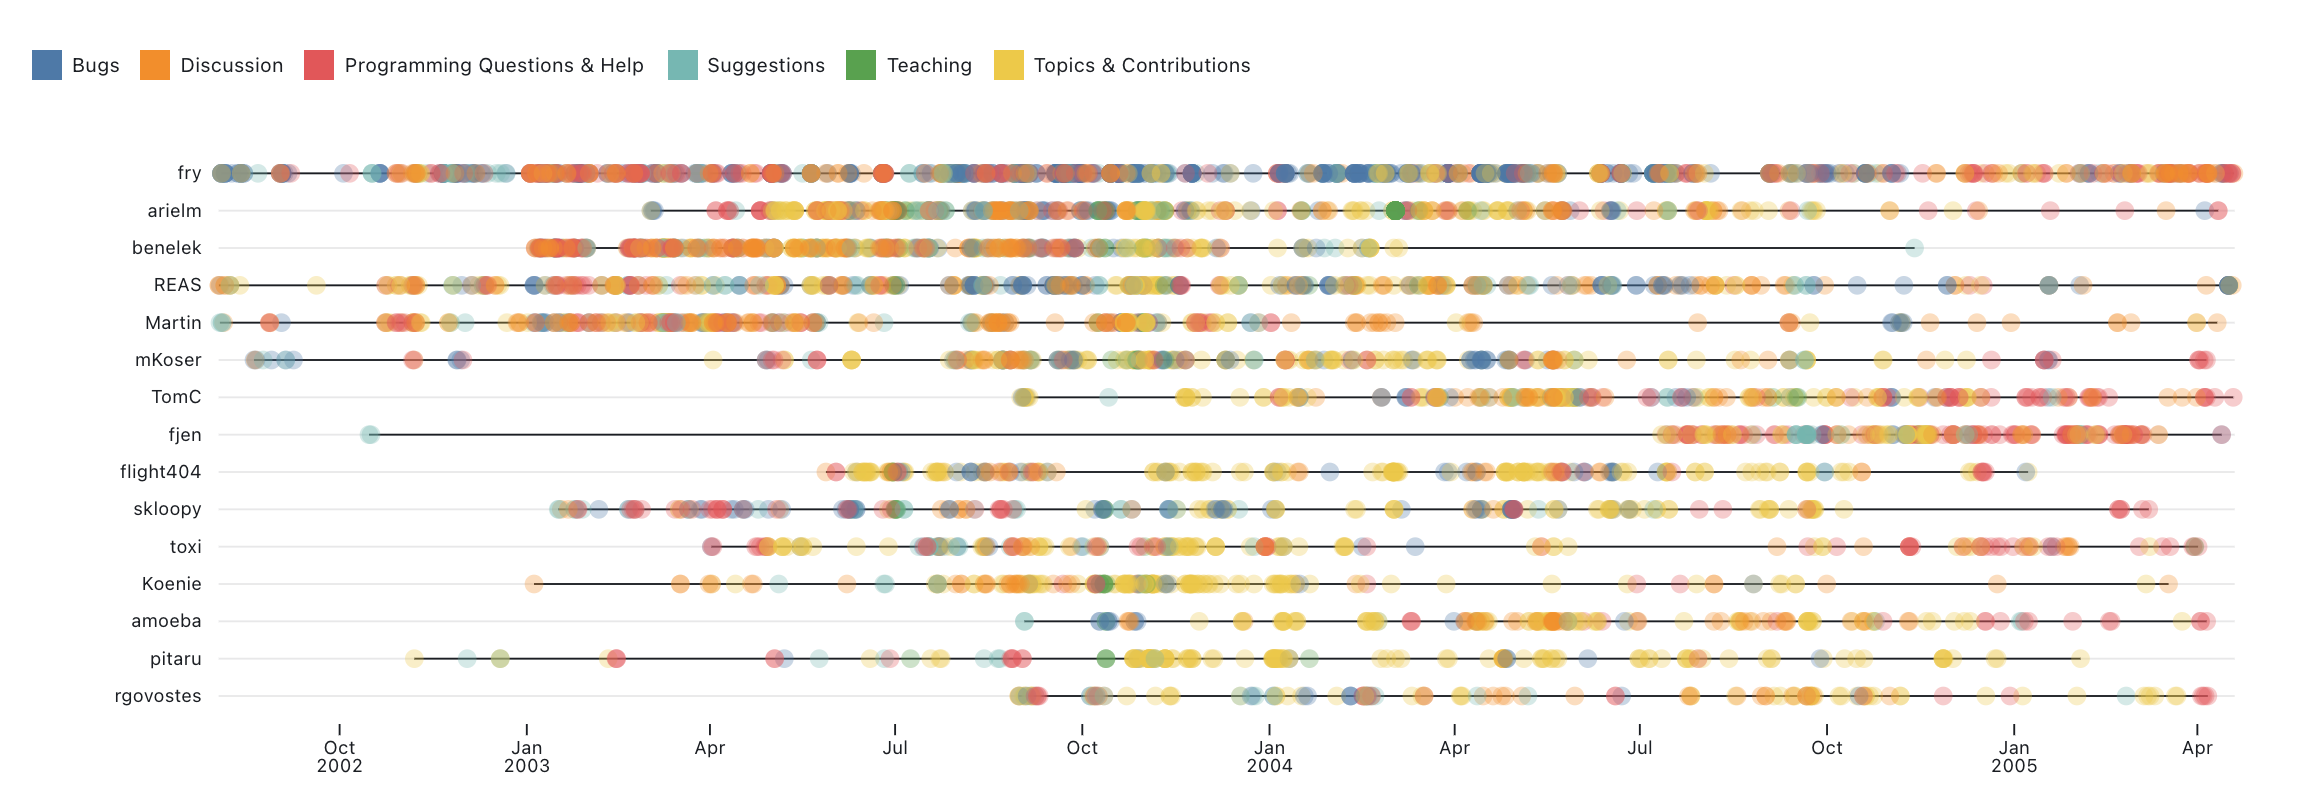
\includegraphics[width=1.0\textwidth]{images/alpha-forum-top15.png}
  \caption{Posting activity of the 15 most active contributors on the alpha forum.}
  \label{fig:processing-alpha-dot}
\end{figure}

Linus's Law—"Given enough eyeballs, all bugs are shallow" \parencite[29]{raymondCathedralBazaar1999}—is somewhat evidenced by increased forum activity during release periods, suggesting community involvement in bug identification, as demonstrated in Figure~\ref{figure:forum-git-activity}.

\begin{figure}[!htbp] 
    \centering 
    %\includesvg[pretex=\sffamily\fontsize{5.58pt}{8pt}\selectfont, width=1\textwidth, keepaspectratio]{images/figure-forum-git-activity.png}
    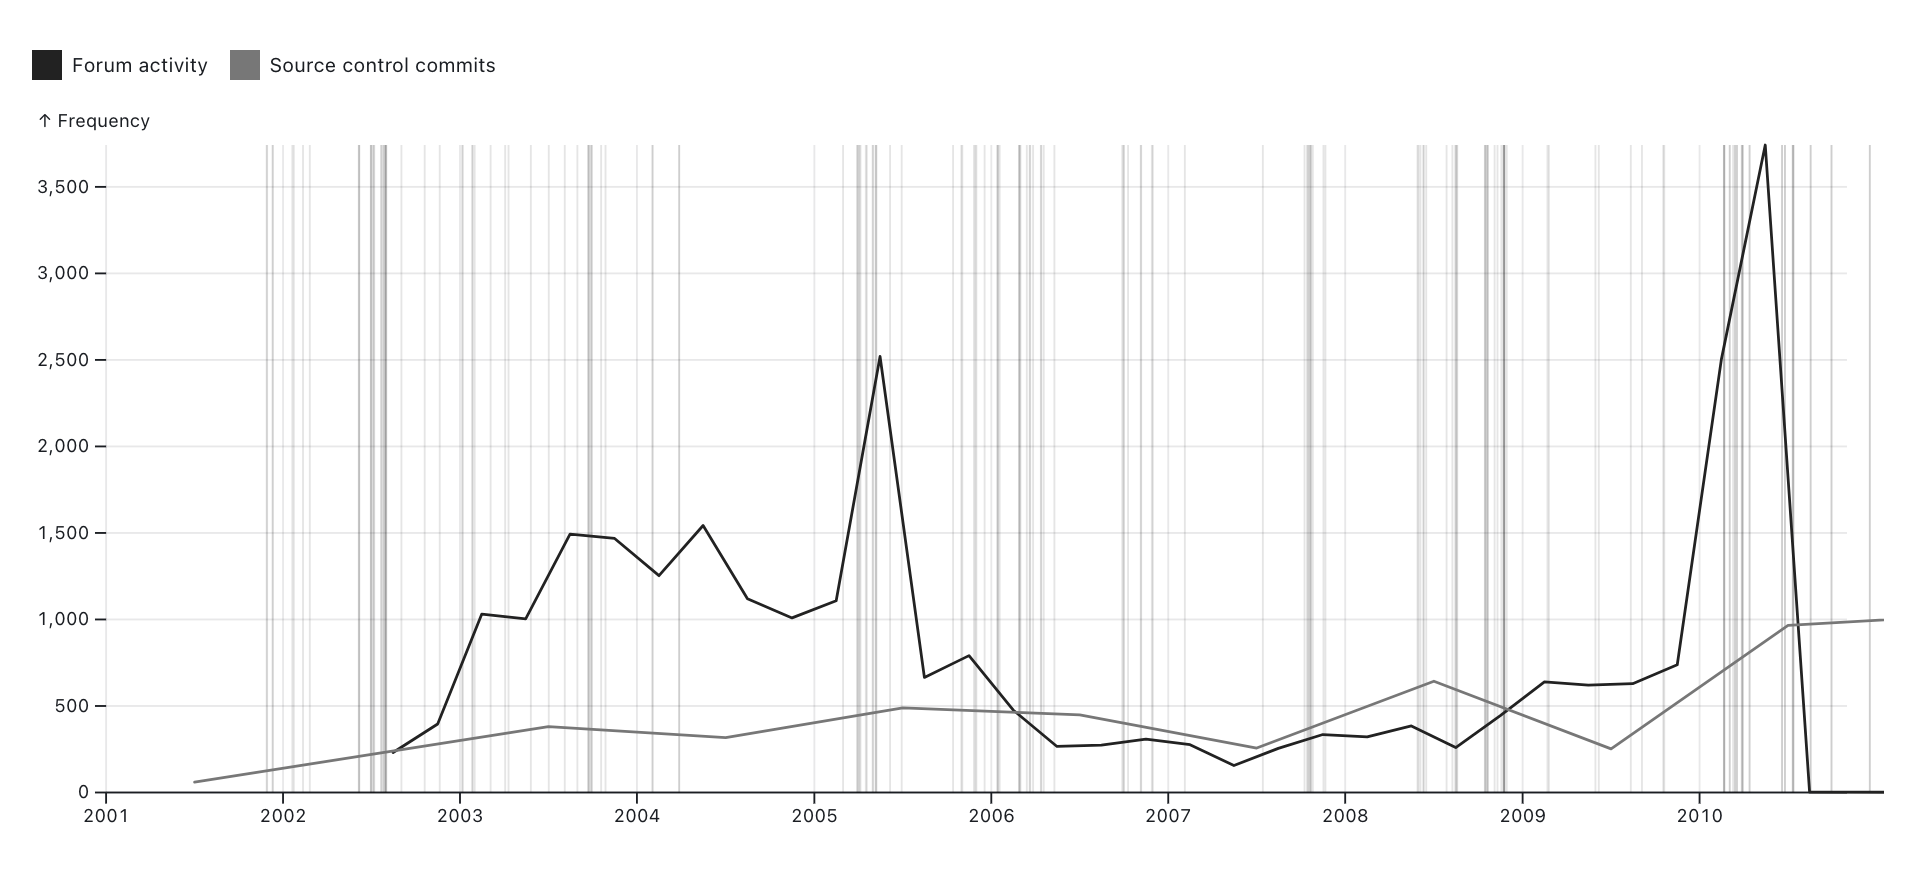
\includegraphics[width=1\textwidth]{images/figure-forum-git-activity.png} 

    \caption{Forum vs git activity vs releases (vertical lines)}
    \label{figure:forum-git-activity}  
  \end{figure}

Contrary to the initial assumption that primary contributors would predominantly be from the MIT ACG group, given the project's origins, a preliminary analysis suggests otherwise.

\begin{figure}[htbp]
  \centering
  
  % Row 1
  \begin{subfigure}[b]{0.24\textwidth}
      \includesvg[pretex=\sffamily\fontsize{5.58pt}{8pt}\selectfont, width=1\textwidth, keepaspectratio]{images/month1.svg}
      \caption{Month 1}
      \label{fig:month1}
  \end{subfigure}
  \hfill
  \begin{subfigure}[b]{0.24\textwidth}
    \includesvg[pretex=\sffamily\fontsize{5.58pt}{8pt}\selectfont, width=1\textwidth, keepaspectratio]{images/month2.svg}
      \caption{Month 2}
      \label{fig:month2}
  \end{subfigure}
  \hfill
  \begin{subfigure}[b]{0.24\textwidth}
    \includesvg[pretex=\sffamily\fontsize{5.58pt}{8pt}\selectfont, width=1\textwidth, keepaspectratio]{images/month3.svg}
      \caption{Month 3}
      \label{fig:month3}
  \end{subfigure}
  \hfill
  \begin{subfigure}[b]{0.24\textwidth}
    \includesvg[pretex=\sffamily\fontsize{5.58pt}{8pt}\selectfont, width=1\textwidth, keepaspectratio]{images/month4.svg}
      \caption{Month 4}
      \label{fig:month4}
  \end{subfigure}
  
  % Add space between rows
  \vspace{0.25cm}

  % Row 2
  \begin{subfigure}[b]{0.24\textwidth}
    \includesvg[pretex=\sffamily\fontsize{5.58pt}{8pt}\selectfont, width=1\textwidth, keepaspectratio]{images/month5.svg}
      \caption{Month 5}
      \label{fig:month5}
  \end{subfigure}
  \hfill
  \begin{subfigure}[b]{0.24\textwidth}
    \includesvg[pretex=\sffamily\fontsize{5.58pt}{8pt}\selectfont, width=1\textwidth, keepaspectratio]{images/month6.svg}
      \caption{Month 6}
      \label{fig:month6}
  \end{subfigure}
  \hfill
  \begin{subfigure}[b]{0.24\textwidth}
    \includesvg[pretex=\sffamily\fontsize{5.58pt}{8pt}\selectfont, width=1\textwidth, keepaspectratio]{images/month7.svg}
      \caption{Month 7}
      \label{fig:month 7}
  \end{subfigure}
  \hfill
  \begin{subfigure}[b]{0.24\textwidth}
    \includesvg[pretex=\sffamily\fontsize{5.58pt}{8pt}\selectfont, width=1\textwidth, keepaspectratio]{images/month8.svg}
      \caption{Month 8}
      \label{fig:month 8}
  \end{subfigure}

  % Add space between rows
  \vspace{0.25cm}

  % Row 3
  \begin{subfigure}[b]{0.24\textwidth}
    \includesvg[pretex=\sffamily\fontsize{5.58pt}{8pt}\selectfont, width=1\textwidth, keepaspectratio]{images/month9.svg}
      \caption{Month 9}
      \label{fig:month9}
  \end{subfigure}
  \hfill
  \begin{subfigure}[b]{0.24\textwidth}
    \includesvg[pretex=\sffamily\fontsize{5.58pt}{8pt}\selectfont, width=1\textwidth, keepaspectratio]{images/month10.svg}
      \caption{Month 10}
      \label{fig:month10}
  \end{subfigure}
  \hfill
  \begin{subfigure}[b]{0.24\textwidth}
    \includesvg[pretex=\sffamily\fontsize{5.58pt}{8pt}\selectfont, width=1\textwidth, keepaspectratio]{images/month11.svg}
      \caption{Month 11}
      \label{fig:month11}
  \end{subfigure}
  \hfill
  \begin{subfigure}[b]{0.24\textwidth}
    \includesvg[pretex=\sffamily\fontsize{5.58pt}{8pt}\selectfont, width=1\textwidth, keepaspectratio]{images/month12.svg}
      \caption{Month 12}
      \label{fig:month12}
  \end{subfigure}
  
  \caption{Monthly graphs}
  \label{fig:monthlyGraphs}
\end{figure}


\begin{figure}[h!] 
  \centering 
  \includesvg[pretex=\sffamily\fontsize{5.58pt}{8pt}\selectfont, width=1\textwidth, keepaspectratio]{images/year.svg}
  \caption{Year}
  \label{figure:year}  
\end{figure}


%\begin{figure}[h!] 
    \centering 
    \includesvg[pretex=\sffamily\fontsize{5.58pt}{8pt}\selectfont, width=1\textwidth, keepaspectratio]{images/figure-forum-posts.svg}
    \caption{Top 12 authors by number of posts (Aggregated alpha and beta forum)}
    \label{fig:forum-posts}  
  \end{figure}

%\begin{figure}[htbp] 
    \centering
    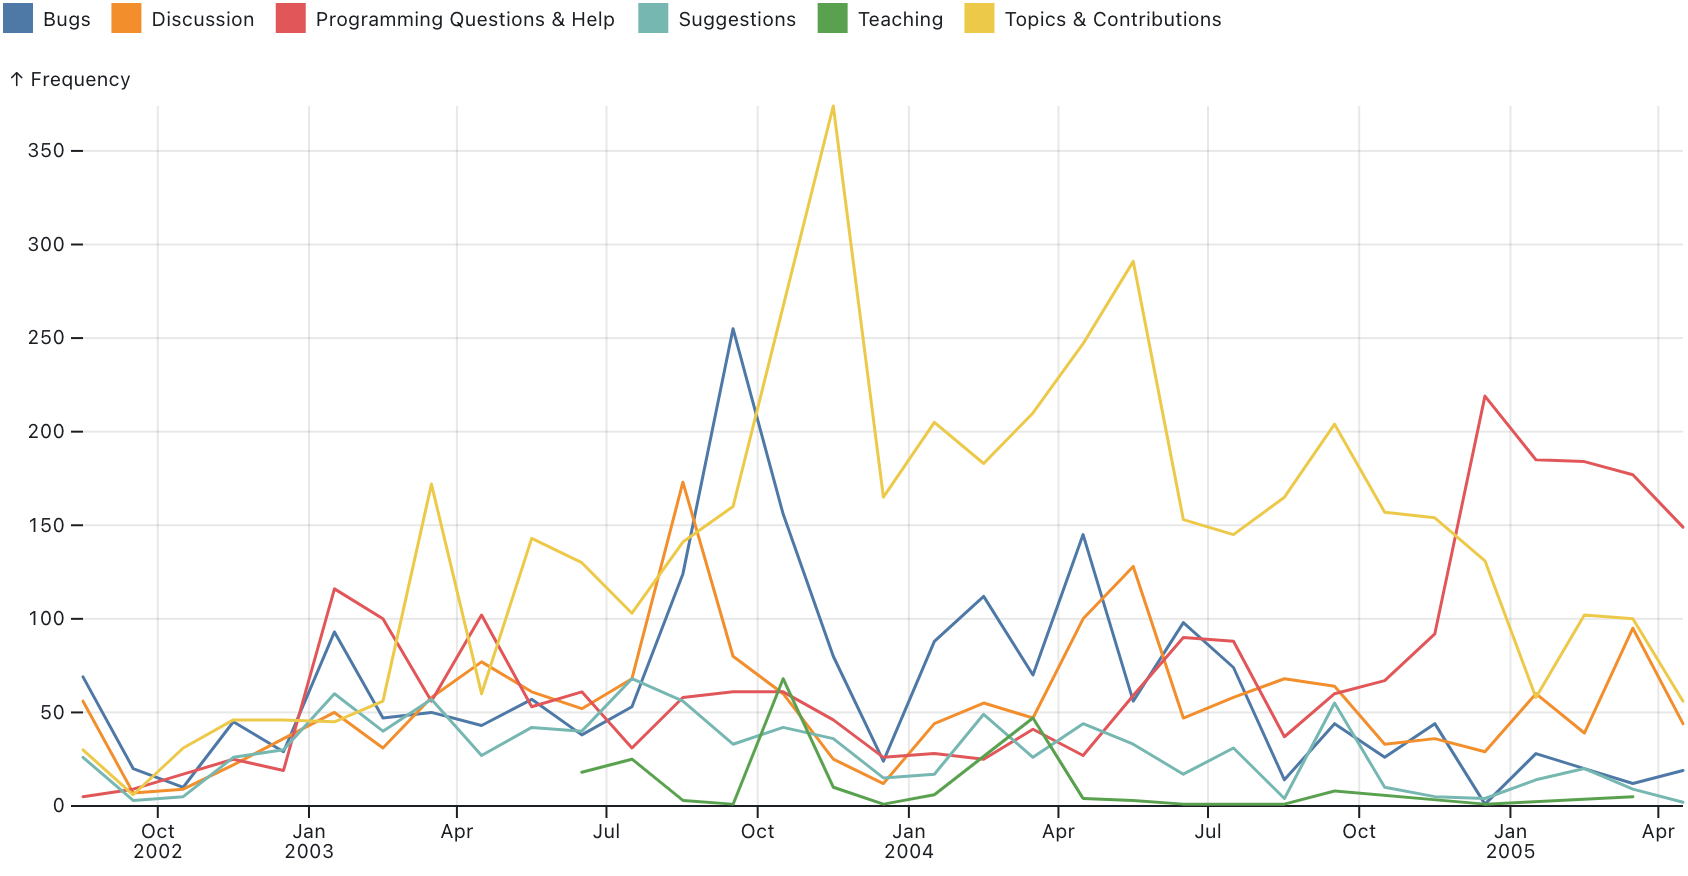
\includegraphics[width=1\textwidth]{alpha-forums-activity.png} 
    % \includesvg[pretex=\sffamily\fontsize{5.58pt}{8pt}\selectfont, width=0.6\textwidth]{images/alpha-forums-activity.svg}
    \caption{Forums activity}
    \label{fig:forum-activity}  
  \end{figure}

%\begin{figure}[h!] 
    \centering 
    \includesvg[pretex=\sffamily\fontsize{5.58pt}{8pt}\selectfont, width=1\textwidth, keepaspectratio]{images/figure-alltime-sourcecode-commits.svg}
    \caption{Top 25 source code contributors by number of commits}
    \label{fig:alltime-sourcecode-commits}  
  \end{figure}

%\begin{figure}[htbp] 
    \centering
    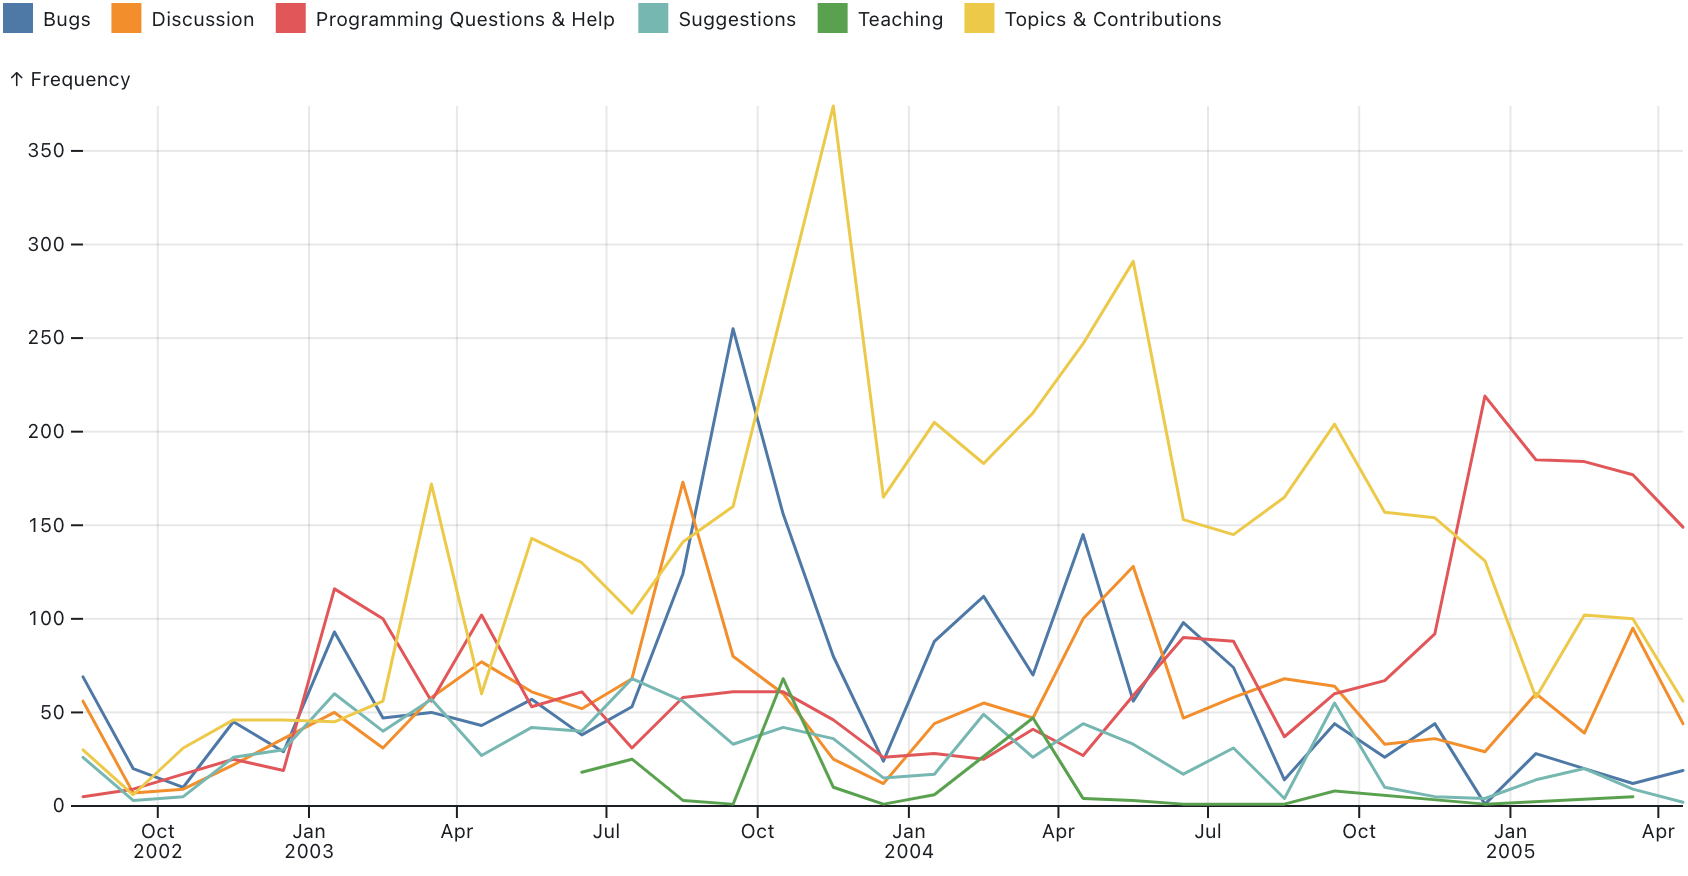
\includegraphics[width=1\textwidth]{alpha-forums-activity.png} 
    % \includesvg[pretex=\sffamily\fontsize{5.58pt}{8pt}\selectfont, width=0.6\textwidth]{images/alpha-forums-activity.svg}
    \caption{Forums activity}
    \label{fig:forum-activity}  
  \end{figure}

% \subsubsection{Synthesized Data Analysis: Git Commits, Releases, and Forum Activity}

\newpage
\subsubsection{Alpha Forum Patterns in Forum Contributions (to remove)}
There were 11,926 posts across 2,626 topics from 02/08/2002, 15:29 to the 19/04/2005, 09:55 across 1039 authors in the forum.

The alpha forum was a YaBB (Yet another Bulletin Board), it was seperated into forums which conained boards which contained topics which contained posts.

\begin{figure}
    \centering 
    \includesvg[pretex=\sffamily\fontsize{5.58pt}{8pt}\selectfont, width=1\textwidth, keepaspectratio]{images/alpha-forums-by-posts.svg}
    \caption{Topics by post number}
    \label{fig:forums}  
  \end{figure}

% todo add
% \subsection{Qualitative Insights}
% \subsubsection{Themes from the Forum}
% \subsubsection{Interview Highlights and Key Takeaways}

% \section{Discussion}

% \subsection{Integrating Quantitative and Qualitative Findings}
% \subsection{Implications for the Open Source Community}
% \subsection{The Unique Case of Processing and Creative Coding}
% \subsection{Limitations of the Study}

% \section{Conclusion and Recommendations}

% \subsection{Recap of Key Findings}
% \subsection{Practical Implications for Open Source Projects}
% \subsection{Recommendations for Future Research}

\section{Acknowledgements}
I'm grateful to Randall Munroe of XKCD for his insightful and humorous comic strips. The comic "Dependency" from \getyear{munroeDependency2020} is in Figure~\ref{fig:dependency_comic} and cited as~\cite{munroeDependency2020}. It's under the Creative Commons Attribution-NonCommercial 2.5 License (CC BY-NC 2.5). License details: \url{https://creativecommons.org/licenses/by-nc/2.5/}.

\section{Bibliography}
\printbibliography

\section{Appendices}

\subsection{Interview Transcripts}

\section*{Interview Guide for Core Contributor}

\subsection*{Perceptions of Expertise and Community Role}

\begin{enumerate}
    \item Has your consistent involvement in resolving technical queries cultivated a sense of expertise or personal satisfaction for you?
    \item Can you comment on the emotional or psychological rewards, if any, you get from contributing?
    \item If you ceased your contributions tomorrow, what implications do you think that would have on the Processing project?
\end{enumerate}

\subsection*{Social Dynamics within the Community}

\begin{enumerate}[resume]
    \item How would you characterize the social fabric of the Processing community?
    \item Can you share an instance where the community's collective efforts resulted in something you alone couldn't have achieved?
    \item Have you ever experienced any conflicts within the community, and how were they resolved?
\end{enumerate}

\subsection*{Views on Technology and Development}

\begin{enumerate}[resume]
    \item What are your opinions on Flash and other proprietary technologies as they relate to Processing?
    \item Your contributions to Processing have been notably consistent. How do you interpret the fluctuating participation rates from others?
\end{enumerate}

\subsection*{Community and Open Source Development}

\begin{enumerate}[resume]
    \item What has been your observation regarding the community's growth, particularly concerning contributions to open source?
    \item Can you recall any "eureka moments" that significantly influenced the community's direction or ethos?
\end{enumerate}

\subsection*{Legacy and Continuation}

\begin{enumerate}[resume]
    \item How did p5 come into being as a continuation or evolution of Processing?
    \item What role did early literature play in legitimizing or boosting the project? Do you recall the impact of O'Reilly books or other publications?
\end{enumerate}

\section*{Interview Guide for Library Contributor}

\subsection*{Introduction and Motivation}

\begin{enumerate}
    \item What problem prompted you to contribute to Processing?
    \item How did you first hear about and decide to engage with the Processing community?
\end{enumerate}

\subsection*{Social Dynamics and Collaboration}

\begin{enumerate}[resume]
    \item Have you collaborated with other community members? What was that experience like?
    \item Were there any challenges in aligning your contributions with the broader community objectives?
\end{enumerate}
\subsection{Data Collection Tools and Scripts}

\begin{itemize}
    \item \href{https://forum.processing.org/alpha/}{Processing Alpha Forum}
    \item \href{https://observablehq.com/d/042b1cf42ea9bb5e}{Observable Notebook for Forum Analysis}
\end{itemize}


% \subsection{List of Forum Threads Analyzed}


\end{document}